\setcounter{exercisegroup}{7}
\edef\CurrentExerciseGroup{\arabic{exercisegroup}}
\section*{\texorpdfstring{\S\CurrentExerciseGroup}{第{\CurrentExerciseGroup}节}}
\phantomsection
\addcontentsline{toc}{section}{第{\CurrentExerciseGroup}节习题}

\begin{enumerate}
\def\labelenumi{\arabic{enumi})}
\tightlist
\item
  \begin{enumerate}
  \def\labelenumii{\alph{enumii})}
  \tightlist
  \item
    设 \(\mathbf{K}\) 是 Hausdorff 局部凸空间 \(\mathbf{E}\) 的一个紧凸子集，\(\mu\) 是 \(\mathbf{K}\) 上质量为 1 的一个正测度，\(\mathbf{b}_{\mu}\) 是它的重心。试证：对每个正函数 \(f\) （\(\mathbf{K}\) 上的、凹的下半连续者），有 \(f(\mathbf{b}_{\mu}) \geqslant \int^{*} f d\mu\) 。（注意 \(f\) 有界（TVS, II, §2 习题 32），因而 \(-f\) 是 \(\mu\) -可积的。）由此推出：若 \(f\) 是 \(\mathbf{K}\) 上既凸又凹的下半连续（或上半连续）函数，则 \(\int f d\mu = f(\mathbf{b}_{\mu})\) 。
  \end{enumerate}
\end{enumerate}

\begin{enumerate}
\def\labelenumi{\alph{enumi})}
\setcounter{enumi}{1}
\tightlist
\item
  设 I 是 R 中的区间 \([0,1]\) ，K 是 \(\mathcal{M}_{+}(I)\) 中由总质量为 1 的正测度所组成的子集，它对淡拓扑是凸的且紧的，并设 \(j: x \mapsto \varepsilon_{x}\) 是 I 到 K 中的典范单射，它是 I 到 K 的一个子空间上的同胚。对每个测度 \(\nu \in K\) ，令 \(g(\nu) = \sum_{x \in I} \nu(\{x\})\) ；这是一个
\end{enumerate}

在 K 中既凸又凹的函数；此外，若 \(g_{n}(\nu)\) 是对 I 的至多含 n 个元素的所有有限子集 A 取的诸 \(\nu(A)\) 的上确界，则 \(g_{n}\) 在 K 上上半连续，且 \(g(\nu) = \lim_{n \to \infty} g_{n}(\nu)\) 对每个 \(\nu \in K\) 成立，因此 g 对 K 上每个测度 \(\lambda\) 都是 \(\lambda\) -可积的。设 \(\mu\) 是 K 上满足 \(\int f d\mu = \int_{\mathrm{I}} f(j(x)) dx\) （对 \(f \in \mathcal{K}(\mathrm{X}; \mathbf{R})\) ）的测度，它是正的且总质量为 1；试证 \(\mathbf{b}_{\mu}\) 是 I 上的 Lebesgue 测度，且 \(\int g d\mu \neq g(\mathbf{b}_{\mu})\) 。

\begin{enumerate}
\def\labelenumi{\arabic{enumi})}
\setcounter{enumi}{1}
\tightlist
\item
  设 X 是紧空间，P 是 X 上取值于 \(]-\infty,+\infty]\) 的下半连续数值函数所成的集。假定 P 包含有限常数；对每个函数 \(h\in P\) 及 X 上每个正测度 \(\mu\) ，\(\mu^{*}(h)\) 有定义且 \(>-\infty\) （§4 习题 5）。
\end{enumerate}

\begin{enumerate}
\def\labelenumi{\alph{enumi})}
\item
  对两个正测度 \(\mu, \nu\) （\(X\) 上的），把 \(\mu \prec \nu\) 定义为：\(\mu^{*}(h) \leqslant \nu^{*}(h)\) 对每个函数 \(h \in \mathcal{P}\) 成立。试证关系 \(\mu \prec \nu\) 是 \(\mathcal{M}_{+}(X)\) 上的一个预序关系；它蕴涵 \(\mu(1) = \nu(1)\) 、\(c\mu \prec c\nu\) （对一切 \(c > 0\) ），以及 \(\mu + \lambda \prec \nu + \lambda\) 对每个测度 \(\lambda \in \mathcal{M}_{+}(X)\) 成立。
\item
  假定 \(\mathcal{P} + \mathcal{P} \subset \mathcal{P}\) ，且 \(c \cdot \mathcal{P} \subset \mathcal{P}\) 对 \(c > 0\) 成立。设 \(\mu\) 是 \(X\) 上一个正测度，\(f\) 是 \(\mathcal{C}(X; \mathbf{R})\) 中一个函数。用 \(Q_f\) 表示函数 \(h \geqslant f\) （\(\mathcal{P}\) 中的）所成的集，用 \(M_\mu\) 表示测度 \(\lambda \in \mathcal{M}_+(X)\) （满足 \(\lambda \prec \mu\) 者）所成的集。试证
\end{enumerate}

\[
\sup _ {\lambda \in \mathrm{M} _ {\mu}} \lambda (f) = \inf _ {h \in \mathrm{Q} _ {f}} \mu^ {*} (h).
\]

（对每个函数 \(g \in \mathcal{C}(\mathrm{X};\mathbf{R})\) ，令 \(p(g) = \inf_{h \in \mathrm{Q}_g} \mu^*(h)\) 。试证：\(p(g + g') \leqslant p(g) + p(g')\) 与 \(p(cg) = c \cdot p(g)\) 对 \(g, g'\) （\(\mathcal{C}(\mathrm{X};\mathbf{R})\) 中的）及 \(c > 0\) 成立；另一方面证明 \(\mathrm{M}_{\mu}\) 恰与满足下列条件的测度 \(\lambda \in \mathcal{M}_{+}(\mathrm{X})\) 所成之集相同：对每个函数 \(g \in \mathcal{C}(\mathrm{X};\mathbf{R})\) 有 \(\lambda(g) \leqslant p(g)\) ，然后应用 Hahn-Banach 定理得出结论。）若 \(\mathcal{P}\) 中函数连续且 \(S_0(f)\) 是 \(Q_f\) 的下包络，则也有 \(\mu(S_0(f)) = \sup \lambda(f)\) 。

\[
\lambda \in \mathrm{M} _ {\mu}
\]

\begin{enumerate}
\def\labelenumi{\alph{enumi})}
\setcounter{enumi}{2}
\item
  若集 \(\mathcal{P}_0\) （由 \(\mathcal{P}\) 中在 X 上连续且有限的函数组成）在 \(\mathcal{C}(\mathrm{X};\mathbf{R})\) 中完全，则关系 \(\mu \prec \nu\) 是 \(\mathcal{M}_{+}(\mathrm{X})\) 上的一个序关系。若测度 \(\nu \in \mathcal{M}_{+}(\mathrm{X})\) 对此序关系是极大的，则每个测度 \(\nu'\) （满足 \(0 \leqslant \nu' \leqslant \nu\) 者，对通常的序）也是极大的（用反证法并利用 \(a\) )）。若 \(\mathcal{P}_0 = \mathcal{P}\) 且 \(\mathcal{P}\) 完全，则关于序关系 \(\mu \prec \nu\) 的每个递增有向集对此关系在 \(\mathcal{M}_{+}(\mathrm{X})\) 中有上确界；特别地，\(\mathcal{M}_{+}(\mathrm{X})\) 对此关系是归纳的。
\item
  假定 \(\mathcal{P}\) 中函数连续且有限，\(\mathcal{P}\) 在 \(\mathcal{C}(\mathrm{X};\mathbf{R})\) 中完全，且 \(\mathcal{P} + \mathcal{P} \subset \mathcal{P}\) 与 \(c \cdot \mathcal{P} \subset \mathcal{P}\) 对一切 \(c > 0\) 成立。对每个函数 \(f \in \mathcal{C}(\mathrm{X};\mathbf{R})\) ，用 \(\mathrm{S}(f)\) 表示函数 \(h \in -\mathcal{P}\) （满足 \(f \leqslant h\) ）的下包络；对每个 \(\varepsilon > 0\) ，用 \(\mathrm{K}_{f,\varepsilon}\) 表示由 \(x \in \mathrm{X}\) （使 \(\mathrm{S}(f)(x) \geqslant f(x) + \varepsilon\) 者）组成的集。试证下列条件等价：
\end{enumerate}

\(\alpha)\) 测度 \(\mu \in \mathcal{M}_{+}(\mathrm{X})\) 关于序关系 \(\lambda \prec \lambda'\) 是极大的。

\(\beta)\) 对每个函数 \(f \in \mathcal{C}(\mathrm{X}; \mathbf{R})\) ，\(\mu(\mathrm{S}(f)) = \mu(f)\) 。

\(\beta^{\prime})\) 对每个函数 \(f \in \mathcal{P}\) ，\(\mu(\mathrm{S}(f)) = \mu(f)\) 。

\(\gamma)\) 对每个函数 \(f \in \mathcal{C}(\mathrm{X}; \mathbf{R})\) 及每个 \(\varepsilon > 0\) ，\(\mu(\mathrm{K}_{f,\varepsilon}) = 0\) 。

\(\gamma^{\prime})\) 对每个函数 \(f\in \mathcal{P}\) 及每个 \(\varepsilon >0\) ，\(\mu (\mathrm{K}_{f,\varepsilon}) = 0\)

（把 b) 应用于 \(-\mathcal{P}\) 。）

\begin{enumerate}
\def\labelenumi{\alph{enumi})}
\setcounter{enumi}{4}
\tightlist
\item
  在 \(d\) ) 的假设下，试证：若 \(\mu\) 与 \(\mu'\) 是 \(X\) 上对关系 \(\prec\) 极大的两个正测度，则 \(\mu + \mu'\) 亦然。由此推出：对此序关系极大的正测度所成之集对通常的序关系 \(\leqslant\) 是一个格。
\end{enumerate}

¶ 3) 设 X 是非空紧空间，P 是 X 上取值于 \([-\infty, +\infty]\) 的下半连续数值函数所成的集；假定 P 包含有限常数。称点 \(x \in X\) 为 P-极值点，如果测度 \(\varepsilon_{x}\) 关于预序关系 \(\mu \prec \nu (*)\) 是极小的；P-极值点所成之集记作 \(\mathrm{Ch}_{\mathcal{P}}(\mathrm{X})\) 。

\begin{enumerate}
\def\labelenumi{\alph{enumi})}
\tightlist
\item
  试证：若 \(\mathcal{P}'\) 是线性组合 \(\sum_{i} c_i h_i\) （\(\mathcal{P}\) 中函数的）所成之集
\end{enumerate}

（系数 \(\geqslant 0\) ）所成之集，则 \(\mathcal{P}\) -极值点与 \(\mathcal{P}'\) -极值点相同。

\begin{enumerate}
\def\labelenumi{\alph{enumi})}
\setcounter{enumi}{1}
\tightlist
\item
  对点 \(x \in X\) ，试证下列条件等价：
\end{enumerate}

\(\alpha)\) \(x\) 是 \(\mathcal{P}\) -极值点。

\(\beta)\) 对每个函数 \(f \in \mathcal{C}(\mathrm{X}; \mathbf{R})\) 及每个 \(\varepsilon > 0\) ，存在 \(h \in \mathcal{P}'\) 使 \(f \leqslant h\) 且 \(h(x) \leqslant f(x) + \varepsilon\) 。

\(\gamma)\) 对 \(x\) 的每个开邻域 U 及每个 \(\varepsilon > 0\) ，存在函数 \(h \geqslant 0\) 属于 \(\mathcal{P}'\) ，使 \(h(x) \leqslant \varepsilon\) 且 \(h(y) \geqslant 1\) 对一切 \(y \in X - U\) 成立。（利用习题 2 b。）

此外，试证 \(\mathrm{Ch}_{\mathcal{P}}(\mathrm{X})\) 中使 \(\mathcal{P}\) 至少有一个函数在 \(\mathrm{X}\) 达到其下确界的点所成之集在 \(\mathrm{Ch}_{\mathcal{P}}(\mathrm{X})\) 中稠密。

\begin{enumerate}
\def\labelenumi{\alph{enumi})}
\setcounter{enumi}{2}
\item
  称 X 的子集 F 为 P-稳定的，如果它是闭的，且关系 \(\lambda \prec \mu\) 与 \(\operatorname{Supp}(\mu) \subset F\) 蕴涵 \(\operatorname{Supp}(\lambda) \subset F\) 。试证：若 \(u \in P\) 且 \(F'\) 是 F 中使 u 在 F 达到其下确界的点所成之集，则 \(F'\) 是 P-稳定的。
\item
  再假定 \(\mathcal{P}\) 分隔 X 的点。试证：对每个函数 \(h \in \mathcal{P}\) ，集 \(S_h\) （X 中使 \(h\) 在 X 达到其下确界的点所成者）与 \(\mathrm{Ch}_{\mathcal{P}}(X)\) 相交。（考察一个极小 \(\mathcal{P}\) -稳定子集（含于 \(S_h\) 者），并用 \(c\) ) 证明这样的子集化为一点。）
\item
  在与 \(d\) ) 相同的假设下，试证：为使 \(\mathbf{F}\) （\(\mathbf{X}\) 的闭子集）包含 \(\mathrm{Ch}_{\mathcal{P}}(\mathbf{X})\) ，必须且只须对每个函数 \(h \in \mathcal{P}'\) ，\(\mathbf{F}\) 与 \(\mathbf{S}_h\) （使 \(h\) 在 \(\mathbf{X}\) 中达到其下确界的点所成之集）相交（利用 \(b\) )）。由此推出：为使 \(a \in \mathbf{X}\) 属于 \(\mathrm{Ch}_{\mathcal{P}}(\mathbf{X})\) 的闭包，必须且只须对每个开邻域 \(\mathbf{U}\) （含 \(a\) ）都存在 \(h \in \mathcal{P}'\) 与 \(b \in \mathbf{U}\) ，使 \(h(b) < h(x)\) 对一切 \(x \in \mathbf{X} - \mathbf{U}\) 成立（换言之，\(\mathbf{S}_h \subset \mathbf{U}\) ）。
\item
  在 \(d\) ) 的假设下，称 X 的子集 A 为 \(\mathcal{P}\) -边，如果对每个函数 \(h \in \mathcal{P}'\) ，\(\mathrm{S}_h\) 与 A 相交。取 X 为 \(\mathbf{R}^2\) 中以 \((-1,0)\) 与 \((1,0)\) 为心、以 1 为半径的两圆之并，取 \(\mathcal{P}\) 为 \(\mathbf{R}^2\) 上仿射线性函数在 X 上的限制所成之集。试证 \(\operatorname{Ch}_{\mathcal{P}}(\mathrm{X})\) 由 X 的点 \((\xi, \eta)\) （其中 \(|\xi| \geqslant 1\) ）组成。若 \(a\) 是 \(\mathcal{P}\) -极值点 \((1,1)\) ，试证存在 \(a\) 的一个邻域 U，使得没有函数 \(h \in \mathcal{P}'\) 满足 \(h \geqslant 0\) 、\(h(a) = 0\) 且 \(h(y) \geqslant 1\) 在 \(\mathrm{X} - \mathrm{U}\) 上成立。若 A 与 \(\mathrm{A}'\) 分别是 \(\operatorname{Ch}_{\mathcal{P}}(\mathrm{X})\) 中点 \((1,1)\) 与 \((-1,1)\) 的余集，则 A 与 \(\mathrm{A}'\) 都是 \(\mathcal{P}\) -边，但 \(\mathrm{A} \cap \mathrm{A}'\) 则不然；因而不存在最小的 \(\mathcal{P}\) -边。
\end{enumerate}

\(g)\) 设 \(\mathbf{Y}\) 是第二个紧空间，\(\mathcal{Q}\) 是 \(\mathbf{Y}\) 到 \([-\infty, +\infty]\) 中的下半连续映射所成之集，且包含有限常数。设 \(\mathcal{H}\) 为形如 \(h = f \otimes g\) （\(f \in \mathcal{P}\) ，\(g \in \mathcal{Q}\) ）的函数所成之集；试证 \(\mathrm{Ch}_{\mathcal{H}}(\mathrm{X} \times \mathrm{Y}) = \mathrm{Ch}_{\mathcal{P}}(\mathrm{X}) \times \mathrm{Ch}_{\mathcal{Q}}(\mathrm{Y})\) 。

¶ 4) 设 E 是 Hausdorff 局部凸空间，X 是 E 中的紧凸集，P 是在 X 上连续且凸的有限数值函数所成的集；\(\mu \prec \nu\) 表示由 P 在 \(\mathcal{M}_{+}(X)\) 上定义的预序关系（习题 2）。

\begin{enumerate}
\def\labelenumi{\alph{enumi})}
\item
  试证 \(\mu \prec \nu\) 是 \(\mathcal{M}_{+}(\mathrm{X})\) 上的一个序关系（利用 TVS, II, §5 习题 29），并且，对每个 \(x \in \mathrm{X}\) ，关系 \(\varepsilon_x \prec \mu\) 等价于说 \(\mu\) 的质量为 1 且 \(x\) 是 \(\mu\) 的重心。于是，对每个质量为 1 的（关于前述序关系的）极大测度 \(\mu\) ，存在一个且仅一个 \(x \in \mathrm{X}\) 使 \(\varepsilon_x \prec \mu\) 。反之，每个 \(z \in \mathrm{X}\) 都是至少一个极大测度的重心。为使 \(x \in \mathrm{X}\) 是 \(\mathrm{X}\) 的极值点，必须且只须 \(\varepsilon_x\) 是极大测度。
\item
  设 \(\mu\) 是 \(\mathrm{X}\) 上的极大测度，\(f\) 是 \(\mathcal{C}_{+}(\mathrm{X})\) 中的函数。试证：对每个 \(\varepsilon > 0\) ，存在函数 \(g\) 在 \(\mathrm{X}\) 上连续且凸，使 \(0 \leqslant g \leqslant f\) 且 \(\mu(g) \geqslant \mu(f) - \varepsilon\) （利用习题 3 b) 与 2 d)）。由此推出 \(\mu\) 的支集含于 \(\mathrm{X}\) 的极值点所成之集的闭包中。
\item
  设 \(\mu\) 是 \(X\) 上的极大测度，\((f_n)_{n \geqslant 1}\) 是 \(\mathcal{C}_+(X)\) 中函数的递减序列。试证：若对每个极值点 \(x \in X\) 序列 \((f_n(x))\) 趋于 0，则 \(\lim_{n \to \infty} \mu(f_n) = 0\) （利用 \(b\) ) 构造连续凸函数的递减序列 \((g_n)\) ，使 \(0 \leqslant g_n \leqslant f_n\) 与 \(\mu(g_n) \geqslant \mu(f_n) - \varepsilon\) 对一切 \(n\) 成立，并证明序列 \((g_n(y))\) 对每个 \(y \in X\) 趋于 0）。
\item
  由 c) 推出：若 \(A \subset X\) 不含任何极值点，且是 X 的紧子集序列 \((\mathrm{K}_{n})\) 之并，其中每个紧子集都是 X 中开集的可数交，则 \(\mu(\mathrm{A}) = 0\) 对每个极大测度 \(\mu\) 成立。
\item
  设 \(\mathcal{A}\) 是 X 上的连续函数所成的向量空间，这些函数是 E 上连续仿射线性函数在 X 上的限制。关系 \(\lambda \prec \mu\) 蕴含等式 \(\lambda(h) = \mu(h)\) 对每个函数 \(h \in \mathcal{A}\) 成立；对每个函数 \(f \in \mathcal{C}(\mathrm{X};\mathbf{R})\) ，\(\mathrm{S}(f)\) （函数 \(h \in \mathcal{A}\) 中满足 \(f \leqslant h\) 者的下包络）也是函数 \(g \in -\mathcal{P}\) 中满足 \(f \leqslant g\) 者的下包络。对每个 \(x \in X\) ，关系 \(\varepsilon_x \prec \mu\) 等价于 \(h(x) = \langle h, \mu \rangle\) 对一切 \(h \in \mathcal{A}\) 成立；X 的极值点与 \(\mathcal{A}\) -极值点相同。若 \(f \in \mathcal{P}\) ，则对每个 \(x \in X\) ，
\end{enumerate}

\[
\mathrm{S} (f) (x) = \sup _ {\varepsilon_ {x} \prec \mu} \int f (y) d \mu (y)\tag{*}
\]

（利用习题 2 b)）。若只假定 f 在 X 上凸且上半连续，则此公式不一定再成立（用习题 1 b) 的记号，考虑在 I 在 K 中的像上等于 1、而在其余处等于 0 的函数 f）。

\begin{enumerate}
\def\labelenumi{\alph{enumi})}
\setcounter{enumi}{5}
\tightlist
\item
  试证：当把右端限于以 x 为重心的离散测度 \(\mu\) 时，公式 (*) 仍然成立。
\end{enumerate}

¶ 5) 采用习题 4 e) 的记号，设 \(\mathcal{A}'\) 表示赋范空间 \(\mathcal{A}\) 的对偶，并赋以由 \(\mathcal{A}\) 的序结构导出的序结构（第二章，§2）。另一方面，用 C 表示由 \(X \times \{1\}\) 在空间 \(E \times R\) 中生成的以 0 为顶点的凸锥。

\begin{enumerate}
\def\labelenumi{\alph{enumi})}
\tightlist
\item
  试证下列性质等价：
\end{enumerate}

\begin{enumerate}
\def\labelenumi{(\roman{enumi})}
\item
  每个点 \(x \in X\) 都是唯一的、质量为 1 的极大测度 \(\beta_x\) 在 \(X\) 上的重心。
\item
  由 C 生成的向量空间 F，对于以 C 为其 \(\geqslant0\) 元素所成之集的序结构而言是一个格（换言之，X 是一个单形（TVS, II, §2 习题 41））。
\item
  对每个函数 \(f \in \mathcal{P}\) ，\(S(f)\) 既是凹的又是凸的。
\item
  若 \(\mu\) 与 \(\nu\) 是两个极大测度，且 \(\mu(h) = \nu(h)\) 对一切 \(h \in \mathcal{A}\) 成立，则 \(\mu = \nu\) 。
\item
  向量空间 \(\mathcal{A}'\) 是一个 Riesz 空间。
\item
  若 \(f\) 与 \(g\) 是 \(\mathcal{P}\) 中两个函数，则 \(S(f + g) = S(f) + S(g)\) 。
\end{enumerate}

（首先证明 (i) 蕴含下述性质：

\begin{enumerate}
\def\labelenumi{(\roman{enumi})}
\setcounter{enumi}{6}
\tightlist
\item
  映射 \(x \mapsto \beta_{x}\) 只以一种方式延拓为 F 到 \(\mathcal{M}(X)\) 中由极大测度生成的子空间上的双射线性映射，且此映射把 C 变换为极大测度所成的锥。
\end{enumerate}

然后利用习题 2 e) 由 (vii) 推出 (ii)。为从 (ii) 推出 (iii)，利用 Riesz 空间 F 中的分解引理及习题 4 f)。为从 (iii) 推出 (iv)，利用下述事实：若 \(g \in \mathcal{C}(X; \mathbf{R})\) 既凹又凸，则 \(h \in A\) 中使 \(h(x) > g(x)\) 对一切 \(x \in X\) 成立者所成之集是一个递减有向集（TVS, II, §5 命题 6），且以 g 为其下包络；然后应用习题 4 e)。为从 (iv) 推出 (v)，注意借助习题 4 e)，\(A'\) 可等同于 \(\mathcal{M}(X)\) 中由极大测度生成的子空间。为从 (v) 推出 (vi)，应用 Riesz 空间 \(A'\) 中的分解引理及习题 4 f)。最后，为从 (vi) 推出 (i)，考虑映射 \(f \mapsto S(f)(x)\) ，其中 \(f \in P\) ，\(x \in X\) ，并利用习题 4 e)。

\begin{enumerate}
\def\labelenumi{\alph{enumi})}
\setcounter{enumi}{1}
\item
  当 a) 的条件满足时，试证：对每个函数 \(f \in \mathcal{C}(X; \mathbf{R})\) ，映射 \(x \mapsto \beta_x(f)\) 属于 X 上两个上半连续函数之差所成的有界函数集在 X 上一致收敛拓扑下的闭包（利用 P 在 \(\mathcal{C}(X; \mathbf{R})\) 中完全这一事实）；因而该映射对 X 上每个测度可测。*对 X 上每个正测度 \(\mu\) ，唯一使 \(\nu \succ \mu\) 的极大测度由 \(\nu = \int \beta_x d\mu(x)\) 给出（参看第五章）。*
\item
  当 \(a\) ) 的条件满足且 X 此外还是可度量化时，试证：对每个 \(x \in X\) ，\(\beta_x\) 是唯一的正测度 \(\mu\) ，质量为 1、重心为 \(x\) ，且使 \(\mu(X - L) = 0\) ，其中 \(L\) 是极值点所成之集 \(\mathrm{Ch}_{\mathcal{A}}(X)\) （按定理 1 的方式论证）。
\item
  当 a) 的条件满足时，试证下列性质等价：
\end{enumerate}

\(\alpha)\) 集 \(\mathrm{L} = \mathrm{Ch}_{\mathcal{A}}(\mathrm{X})\) 是闭的，换言之 \(\check{\mathrm{S}}_{\mathcal{A}}(\mathrm{X}) = \mathrm{Ch}_{\mathcal{A}}(\mathrm{X})\) 。

\(\beta)\) 对每个函数 \(f \in \mathcal{P}\) ，\(\mathrm{S}(f)\) 在 \(\overline{\mathrm{L}}\) 上的限制连续。

\(\gamma)\) 对每个函数 \(f \in \mathcal{P}\) ，函数 \(S(f)\) 在 \(X\) 上连续。

\(\delta)\) 映射 \(x \mapsto \beta_x\) （X 到 \(\mathcal{M}_+(X)\) 中，赋以淡拓扑）连续。

（为证 \(\alpha\) ) 蕴含 \(\beta\) ) ，注意在 L 中 \(\beta_x = \varepsilon_x\) 。为证 \(\beta\) 蕴含 \(\gamma\) ) ，利用 S(f) 是 \(\mathcal{A}\) 中函数的递减有向集的下包络这一事实（TVS, II, §5 命题 6）、Dini 定理以及习题 3 \(d\) ) 应用于 \(\mathcal{A}\) 中的函数。为证 \(\gamma\) 蕴含 \(\delta\) ，利用习题 4 \(e\) )。最后，为证 \(\delta\) 蕴含 \(\alpha\) ，利用习题 4 \(a\) 。）

¶ 6) 设 X 是非空紧空间，H 是 \(\mathcal{C}(X;R)\) 的包含常数且分离 X 的点的线性子空间。于是，由 H 定义的（习题 2）关系 \(\lambda \prec \mu\) 是一个等价关系，且习题 3 意义下的 H-极值点与第 3 号意义下的 H-极值点相同。

设 \(\mathbf{F}\) 是 \(\mathbf{X}\) 的包含 \(\operatorname{Ch}_{\mathcal{H}}(\mathbf{X})\) 的闭子集；对每个 \(x \in \mathbf{X}\) ，用 \(\mathcal{M}_x^{\mathrm{F}}\) 表示正测度 \(\mu\) （在 \(\mathbf{X}\) 上、总质量为 1、使 \(\varepsilon_x \prec \mu\) 且 \(\operatorname{Supp}(\mu) \subset \mathbf{F}\) ）所成之集；为使 \(\varepsilon_x \in \mathcal{M}_x^{\mathrm{F}}\) ，必须且只须 \(x \in \mathbf{F}\) ；关系 \(x \in \operatorname{Ch}_{\mathcal{H}}(\mathbf{X})\) 等价于 \(\mathcal{M}_x^{\mathrm{F}} = \{\varepsilon_x\}\) 。对每个有界数值函数 \(f\) （定义在 \(\mathbf{F}\) 上）及每个 \(x \in X\) ，令

\[
\overline {{\mathrm{H}}} _ {x} ^ {\mathrm{F}} (f) = \inf _ {f \leqslant h | \mathrm{F}, h \in \mathscr {H}} h (x), \quad \underline {{\mathrm{H}}} _ {x} ^ {\mathrm{F}} (f) = - \overline {{\mathrm{H}}} _ {x} ^ {\mathrm{F}} (- f) = \sup _ {f \geqslant h | \mathrm{F}, h \in \mathscr {H}} h (x),
\]

它们都是有限数。

\begin{enumerate}
\def\labelenumi{\alph{enumi})}
\item
  试证：映射 \(f \mapsto \overline{\mathrm{H}}_x^{\mathrm{F}}(f)\) （\(\mathcal{C}(\mathrm{F};\mathbf{R})\) 到 \(\mathbf{R}\) 中的映射）是递增的、正齐次的且凸的。若 \(h \in \mathcal{H}\) ，则 \(\overline{\mathrm{H}}_x^{\mathrm{F}}(h) = h(x)\) 。
\item
  对每个 \(x \in X\) 、每个测度 \(\mu \in \mathcal{M}_x^{\mathrm{F}}\) 及每个函数 \(f \in \mathcal{C}(\mathrm{F};\mathbf{R})\) ，有 \(\underline{\mathrm{H}}_x^{\mathrm{F}}(f) \leqslant \int f d\mu \leqslant \overline{\mathrm{H}}_x^{\mathrm{F}}(f)\) 。反之，若对函数 \(f_0 \in \mathcal{C}(\mathrm{F};\mathbf{R})\) ，\(\gamma\) 是使 \(\underline{\mathrm{H}}_x^{\mathrm{F}}(f_0) \leqslant \gamma \leqslant \overline{\mathrm{H}}_x^{\mathrm{F}}(f_0)\) 的实数，则存在测度 \(\mu \in \mathcal{M}_x^{\mathrm{F}}\) 使 \(\gamma = \int f_0 d\mu\) 。
\item
  试证：对函数 \(g \in \mathcal{C}(\mathrm{X};\mathbf{R})\) ，下列条件等价：
\end{enumerate}

\(\alpha)\) 对每个 \(x \in X\) 及每个测度 \(\mu \in \mathcal{M}_x^{\mathrm{F}}\) ，有 \(g(x) = \int g d\mu\) 。

\(\beta)\) 对每个 \(x \in \mathrm{X}\) ，\(\underline{\mathrm{H}}_x^{\mathrm{F}}(g|\mathrm{F}) = \overline{\mathrm{H}}_x^{\mathrm{F}}(g|\mathrm{F}) = g(x)\) 。

\(\gamma)\) 对每个 \(\varepsilon > 0\) ，存在两个有限序列 \((h_i'), (h_j'')\) （\(\mathcal{H}\) 中的函数），使得令 \(h' = \sup(h_i')\) ，\(h'' = \inf(h_j'')\) ，就有 \(h' \leqslant g \leqslant h''\) 且 \(h'' - h' \leqslant \varepsilon\) 。

（为证 \(\beta\) ) 蕴含 \(\gamma\) ，按 GT, X, §4 第 1 号命题 2 的方式论证。）

当函数 \(g \in \mathcal{C}(\mathrm{X};\mathbf{R})\) 具有前述等价性质时，称它为 \(\mathcal{H}\) -调和的；\(\mathcal{H}^c\) （\(\mathcal{H}\) -调和函数所成之集）是 \(\mathcal{C}(\mathrm{X};\mathbf{R})\) 的包含 \(\mathcal{H}\) 的闭线性子空间；它与所考虑的闭集 \(\mathrm{F} \supset \mathrm{Ch}_{\mathcal{H}}(\mathrm{X})\) 无关。我们有 \((\mathcal{H}^c)^c = \mathcal{H}^c\) ，且 \(\mathcal{M}_+(\mathrm{X})\) 中由 \(\mathcal{H}^c\) 定义的等价关系与关系 \(\lambda \prec \mu\) （由 \(\mathcal{H}\) 所定义）相同；从而 \(\mathrm{Ch}_{\mathcal{H}^c}(\mathrm{X}) = \mathrm{Ch}_{\mathcal{H}}(\mathrm{X})\) 。映射 \(g \mapsto g|\mathrm{F}\) 是 \(\mathcal{H}^c\) 到它在 \(\mathcal{C}(\mathrm{F};\mathbf{R})\) 中的像上的严格递增等距（因而该像是 \(\mathcal{C}(\mathrm{F};\mathbf{R})\) 的闭子空间）。

\begin{enumerate}
\def\labelenumi{\alph{enumi})}
\setcounter{enumi}{3}
\item
  取 X 为 R 中区间 \([0,1]\) ，取 H 为 R 上二次多项式在 X 上的限制所成的向量空间。试证 \(H^{c}\) 不同于闭包 \(\overline{H}\) （H 在 \(\mathcal{C}(X;R)\) 中的闭包）。
\item
  试证：为使 \(\mathrm{Ch}_{\mathcal{H}}(\mathrm{X}) = \mathrm{X}\) ，必须且只须 \(\mathcal{H}^c = \mathcal{C}(\mathrm{X};\mathbf{R})\) （为证条件是必要的，利用 \(b\) )）。
\item
  试证：若 \(\mathcal{H}\) 是格序的（换言之，是一个 Riesz 空间），则 \(\mathcal{H}^c = \overline{\mathcal{H}}\) 。举出一个 \(\mathcal{H}\) 非格序而 \(\mathcal{H}^c = \overline{\mathcal{H}}\) 的例子。
\item
  设 \(\mathcal{E}_{\mathcal{H}}\) 是 \(\mathcal{C}(\mathrm{X};\mathbf{R})\) 中包含 \(\mathcal{H}\) 的最小闭子集，使 \(\inf (u,v)\) （\(\mathcal{E}_{\mathcal{H}}\) 中任意两个函数的下包络）属于 \(\mathcal{E}_{\mathcal{H}}\) 。试证下列性质等价：
\end{enumerate}

\(\alpha)\) \(f\in \mathcal{E}_{\mathcal{H}}\)

\(\beta)\) 对每个 \(x \in X\) 及每个测度 \(\mu \in \mathcal{M}_x^X\) ，\(\int f d\mu \leqslant f(x)\) ；

\(\gamma)\ \overline{\mathrm{H}}_{x}^{\mathrm{X}}(f) = f(x)\ \text{对于每个 } x \in \mathrm{X};\)

\(\delta)\) 对每个 \(\varepsilon > 0\) ，存在有限序列 \((h_i)\) （\(\mathcal{H}\) 中的函数），使 \(f \leqslant \inf(h_i) \leqslant f + \varepsilon\) 。

（为证 \(\beta\) ) 蕴含 \(\gamma\) ，利用 \(b\) 。）

由此推出 \(\mathcal{E}_{\mathcal{H}}\) 是一个尖凸锥，且 \(\mathcal{E}_{\mathcal{H}} \cap (-\mathcal{E}_{\mathcal{H}}) = \mathcal{H}^c\) 。试证 \(\mathcal{E}_{\mathcal{H}}\) 中每个函数在 \(X\) 中的下确界都在 \(\mathrm{Ch}_{\mathcal{H}}(X)\) 的至少一个点上达到。

¶ 7) 设 Y 是非空紧空间，R 是 \(\mathcal{C}(\mathrm{Y};\mathbf{R})\) 的一个线性子空间，它包含常数、分离 Y 的点且是格序的（换言之，是一个 Riesz 空间）。

\begin{enumerate}
\def\labelenumi{\alph{enumi})}
\tightlist
\item
  设 \(\mathcal{N}\) 是 \(\mathcal{R}\) 的一个极大孤立子空间（第二章，§1 习题 4）；试证存在一个且仅一个点 \(y_0\) ，使正线性形式 \(\varphi : f \mapsto f(y_0)\)
\end{enumerate}

在 \(\mathcal{R}\) 上是格的（第二章，§2 习题 5 b)），且 \(\mathcal{N} = \overline{\varphi}(0)\) 。（为看出 Y 中至少存在一点，使满足 \(f \geqslant 0\) 且属于 \(\mathcal{N}\) 的所有函数在该点为零，用反证法，证明在相反的情形下，顾及 Y 的紧性以及 R 中序关系的定义，将有 N = R。为证明 Y 中使 N 中所有函数都为零的点所成之集 \(Z(N)\) 化为单独一点，利用下述事实：N 是 R 中的一个超平面（第二章，§2 习题 5），以及 R 分离 Y 的点且包含常数。）

\begin{enumerate}
\def\labelenumi{\alph{enumi})}
\setcounter{enumi}{1}
\item
  在 \(a\) ) 的假设下，试证 \(y_0 \in \check{\mathrm{S}}_{\mathcal{R}}(\mathrm{Y})\) 。（令 \(\mathrm{S} = \check{\mathrm{S}}_{\mathcal{R}}(\mathrm{Y})\) ，注意 \(\mathcal{R}'\) （\(\mathcal{C}(\mathrm{S}; \mathbf{R})\) 中由限制到 \(\mathrm{S}\) 上的 \(\mathcal{R}\) 中函数所构成的子空间）作为序向量空间典范地同构于 \(\mathcal{R}\) （习题 6 c)），并且借助 \(f \mapsto f|\mathrm{S}\) 的逆同构，正线性形式 \(f \mapsto f(y_0)\) 给出 \(\mathcal{R}'\) 上的一个格的正线性形式；然后把 \(a\) ) 应用于 \(\mathcal{R}'\) 。）
\item
  对每个孤立子空间 \(\mathcal{N}_0 \neq \mathcal{R}\) ，试证存在极大孤立子空间 \(\mathcal{N} \supset \mathcal{N}_0\) 。（利用下述事实：若一个孤立子空间包含一个常数函数 \(\neq 0\) ，则它等于 \(\mathcal{R}\) 。）
\item
  设 \(\mathbf{Z}\) 是诸集 \(\mathbf{Z}(\mathcal{N})\) （每个都化为一点）之并，其中 \(\mathcal{N}\) 取遍 \(\mathcal{R}\) 的极大孤立子空间所成之集；试证 \(\mathbf{Z} = \check{\mathbf{S}}_{\mathcal{R}}(\mathbf{Y})\) 。（首先证明 \(\mathbf{Z}\) 是闭的，注意若 \(y \notin \mathbb{Z}\) ，则线性形式 \(f \mapsto f(y)\) 在 \(\mathcal{R}\) 上不是格的，从而（利用第二章，§2 习题 5 b)）线性形式 \(f \mapsto f(y')\) 对一切点 \(y'\) （充分接近 \(y\) 者）也不是格的。然后利用第 3 号命题 7，证明每个函数 \(f_0 \in \mathcal{R}\) 的下确界 \(\alpha\) （在 \(\mathbf{Y}\) 中取的）在 \(\mathbf{Z}\) 的至少一个点上达到；为此，令 \(\mathrm{M} = f_0^{-1}(\alpha)\) ，考虑子空间 \(\mathcal{N}_0\) ，它由函数 \(f \in \mathcal{R}\) （形如 \(f_1 - f_2\) ）组成。
\end{enumerate}

\(\mathrm{M} = \overline{f}_0(\alpha)\) ，考虑子空间 \(\mathcal{N}_0\) ，它由函数 \(f \in \mathcal{R}\) （形如 \(f_1 - f_2\) ，其中 \(f_1 \geqslant 0\) ，\(f_2 \geqslant 0\) ，且 \(f_1\) 与 \(f_2\) 在 \(\mathrm{M}\) 上为零）组成；证明 \(\mathcal{N}_0\) 是孤立的，并利用 \(c\) 。）

¶ 8) 一般记号与假设同习题 6，令 \(S = \check{S}_{\mathcal{H}}(X)\) 。称函数 \(f \in \mathcal{C}(S; \mathbf{R})\) 为 \(\mathcal{H}\) -预解的，如果存在函数 \(g \in \mathcal{H}^c\) 使 \(f = g|S\) （此函数届时是唯一的）。

\begin{enumerate}
\def\labelenumi{\alph{enumi})}
\tightlist
\item
  试证：关于函数 \(f \in \mathcal{C}(\mathbf{S};\mathbf{R})\) 的下列条件等价：
\end{enumerate}

\begin{enumerate}
\def\labelenumi{(\roman{enumi})}
\item
  \(f\) 是 \(\mathcal{H}\) -预解的。
\item
  对每个 \(x \in X\) ，\(\underline{\mathrm{H}}_x^{\mathrm{S}}(f) = \overline{\mathrm{H}}_x^{\mathrm{S}}(f)\) 。
\item
  对每个 \(x \in X\) 及每对测度 \(\mu_1, \mu_2\) （属于 \(\mathcal{M}_x^S\) ），有 \(\int f d\mu_1 = \int f d\mu_2\) 。
\end{enumerate}

（利用习题 6 b) 与 c)。）

\begin{enumerate}
\def\labelenumi{\alph{enumi})}
\setcounter{enumi}{1}
\tightlist
\item
  试证下列性质等价：
\end{enumerate}

\begin{enumerate}
\def\labelenumi{(\roman{enumi})}
\item
  每个函数 \(f \in \mathcal{C}(\mathrm{S};\mathbf{R})\) 都是 \(\mathcal{H}\) -预解的。
\item
  对每个 \(x \in X\) 及每个函数 \(f \in \mathcal{C}(\mathrm{S};\mathbf{R})\) ，\(\underline{\mathrm{H}}_x^{\mathrm{S}}(f) = \overline{\mathrm{H}}_x^{\mathrm{S}}(f)\) 。
\item
  集 \(\mathcal{M}_x^{\mathrm{S}}\) 化为单独一个元素。
\item
  集 \(\mathcal{H}^{\tilde{c}}\) 是格序的。
\item
  对每个函数 \(u \in \mathcal{E}_{\mathcal{H}}\) （习题 6 g)），存在最大下界 \(h_u\) （即 \(u\) 在 \(\mathcal{H}^c\) 中的最大下界）。
\end{enumerate}

（为证 (iv) 蕴含 (i)，对 \(\mathcal{H}^c\) 应用习题 7 d)，证明对每个点 \(s \in S\) ，线性形式 \(h \mapsto h(s)\) 在 \(\mathcal{H}^c\) 中是格的；然后利用 Stone 定理及习题 6 c)。为证 (i) 蕴含 (v)，注意 \(\mathcal{H}^c \subset \mathcal{E}_{\mathcal{H}}\) ，并考虑唯一的函数 \(h_u \in \mathcal{H}^c\) ，它使 \(h_u|S = u|S\) 。为证 (v) 蕴含 (iv)，注意若 \(h \in \mathcal{H}^c\) 则 \(-h^{-} = \inf(h,0) \in \mathcal{E}_{\mathcal{H}}\) ，并对 \(u = -h^{-}\) 应用 (v)。）

\begin{enumerate}
\def\labelenumi{\alph{enumi})}
\setcounter{enumi}{2}
\item
  若 \(b\) ) 的条件满足且 \(\gamma_x\) 是 \(\mathcal{M}_x^S\) 的唯一元素，试证映射 \(x \mapsto \gamma_x\) （\(X\) 到 \(\mathcal{M}_+(X)\) 中，赋以淡拓扑）连续；由此推出此时有 \(\mathrm{Ch}_{\mathcal{H}}(X) = \check{\mathrm{S}}_{\mathcal{H}}(X)\) （注意 \(\gamma_x = \varepsilon_x\) 在 \(\mathrm{Ch}_{\mathcal{H}}(X)\) 中成立）。
\item
  为使每个函数 \(f \in \mathcal{C}(\mathrm{S};\mathbf{R})\) 都是在 \(S\) 上的限制（某个函数 \(h \in \mathcal{H}\) 的限制），必须且只须 \(\mathcal{H}\) 在 \(\mathcal{C}(\mathrm{X};\mathbf{R})\) 中是闭的且是格序的。
\end{enumerate}

\begin{enumerate}
\def\labelenumi{\arabic{enumi})}
\setcounter{enumi}{8}
\tightlist
\item
  设 Y 是这样一个拓扑空间，其底集为乘积 \(I \times \{-1,0,1\}\) （在 \(R^{2}\) 中），其中 \(I = [0,1]\) ；对每个 \(a \in I\) 及每个 \(\varepsilon > 0\) ，令 \(U_{a,\varepsilon}\) 为由 \((x,y) \in Y\) （满足 \(|x - a| \leqslant \varepsilon\) 且 \((x,y)\) 异于 \((a,1)\) 与 \((a,-1)\) ）组成的集；诸集 \(\{(x,y)\}\) （\(y \neq 0\) 且 \(x \in I\) ）与诸集 \(U_{a,\varepsilon}\) 一起构成 Y 上一个拓扑的基，对此拓扑 Y 是一个不可度量化的紧空间（参看 GT, IX, §2 习题 13 d)）。用 X 表示 Y 与一个化为单点 \(\omega\) 的集的拓扑和空间。设 \(\mathcal{H}\) 为 X 上满足下式的连续有限数值函数 \(h\) 所成之集：
\end{enumerate}

\[
h (x, 0) = \frac {1}{2} \bigl (h (x, 1) + h (x, - 1) \bigr)
\]

对一切 \(x \in I\) 成立，且 \(h(\omega) = \int_0^1 h(x, 0) dx\) 。试证 \(\operatorname{Ch}_{\mathcal{H}}(X)\) 由点 \((x, y)\) （满足 \(y \neq 0\) 且 \(x \in I\) ）组成，但不存在 X 上质量为 1 的正测度 \(\mu\) 使 \(h(\omega) = \mu(h)\) 对一切 \(h \in \mathcal{H}\) 成立且 \(\mu(X - \operatorname{Ch}_{\mathcal{H}}(X)) = 0\) 。

¶ 10) a) 设 E 是 Hausdorff 完备局部凸空间，E′ 是其对偶，E′* ⊃ E 是 E′ 的代数对偶。设 A 是 E 的一个子集，它在弱化拓扑 σ(E, E′) 下是紧的。设 x 是 E′* 中的一点，属于 A 的凸包络 C 在弱拓扑 σ(E′,E′) 下的闭包。试证：若 \((x'_n)\) 是 E′ 中点的序列，在弱拓扑 σ(E′,E) 下收敛于 a′ ∈ E′，则 \(\lim_{n \to \infty}\langle x, x'_n\rangle = \langle x, a'\rangle\)。

（注意 \(x\) 是 A 上一个质量为 1 的测度的重心，并应用 Lebesgue 定理。）

\begin{enumerate}
\def\labelenumi{\alph{enumi})}
\setcounter{enumi}{1}
\item
  由 a) 推出：若 E 中存在一个在原拓扑下稠密的点序列，则限制到每个等度连续子集 \(H'\) （\(E'\) 的）上后，映射 \(x' \mapsto \langle x, x' \rangle\) 对弱拓扑 \(\sigma(\mathrm{E}', \mathrm{E})\) 连续（注意 \(H'\) 上由 \(\sigma(\mathrm{E}', \mathrm{E})\) 诱导的拓扑是可度量化的）。由此推出，此时必有 \(x \in E\) （TVS, IV, §5 第 5 号）；换言之，E 中一个在弱化拓扑下紧的集的闭凸包络对该拓扑仍然是紧的。
\item
  把 \(b\) ) 的结果推广到 \(E\) 是任意拟完备 Hausdorff 局部凸空间的情形（Krein 定理）。（首先化归为 \(E\) 是完备空间的情形，这通过考虑 \(\widehat{E}\) 实现；然后注意，凭 Eberlein 定理（TVS, IV, §5 第 3 号定理 1），只需证明每个序列 \((x_n)\) （\(C\) 中的点组成的）在 \(E\) 中对 \(\sigma(E, E')\) 有一个聚点；这就可化归为在 \(E\) 中存在一个原拓扑下稠密的序列的情形。）
\end{enumerate}

\chapter{测度的积分}

本章中，T 表示一个局部紧空间，\(\mu\) 表示 T 上一个正测度。对集 E 的每个子集 A，\(\varphi_{A}\) 表示 A 的特征函数（若不致混淆）。所谓数值函数，我们总指取值于 \(\overline{R}\) 的函数，因而可能取值 \(+\infty\) 与 \(-\infty\) 。定义在 E 上的正数值函数所成之集记作 \(\mathcal{F}_{+}(E)\) ，若不致混淆也简记作 \(F_{+}\) 。我们约定把乘积 \(0 \cdot (+\infty)\) 与 \(0 \cdot (-\infty)\) 定义为取值 0；于是，若 f 是定义在 E 上的数值函数而 A 是 E 的子集，则 \(f\varphi_{A}\) 表示在 A 上与 f 相同、在 CA 上等于 0 的函数。对局部紧空间的每个点 a，\(\varepsilon_{a}\) 表示在点 a 放置单位质量所定义的测度（第三章，§1 第 3 号）。

本质上积分（相应地，本质可积函数）的概念将在 §1 中定义；我们将看到，当局部紧空间 T 在无穷远处可数时（GT, I, §9 第 9 号），它与上积分（相应地，可积函数）的概念一致。

因此，只关心在无穷远处可数的局部紧空间上的积分的读者可以略去 §1 的第 1 至 3 号不读；在本章其余部分，当所考虑的空间在无穷远处可数时，只要删去“本质的”与“本质上”等词，并把记号 \(\mu^{\bullet}\) 换成 \(\mu^{*}\) 、记号 \(\int^{\bullet}\) 换成 \(\int^{*}\) ，就得到有效的命题。

在 §1 至 §4 中，测度一词总是指正测度；其他测度将视情形明确地称为未必正的测度或复测度。

\section{本质上积分}

\subsection{本质上积分的定义}

定义 1. --- 对每个函数 \(f \in \mathcal{F}_{+}(\mathrm{T})\) ，把 \(f\) 关于 \(\mu\) 的本质上积分（记作 \(\mu^{\bullet}(f)\) ）定义为数 \(\mu^{*}(f\varphi_{\mathrm{K}})\) （其中 \(\mathrm{K}\) 取遍 \(\mathrm{T}\) 的一切紧子集）所成之集的上确界（有限或否）。设 \(\mathrm{A}\) 是 \(\mathrm{T}\) 的任意子集，令 \(\mu^{\bullet}(\mathrm{A}) = \mu^{\bullet}(\varphi_{\mathrm{A}})\) 。

也使用记号 \(\int^{\bullet}f d\mu ,\int^{\bullet}f(t)d\mu (t),\int^{\bullet}f\mu\) 。

由于 \(f\varphi_{\mathrm{K}} \leqslant f\) 对每个紧子集 \(\mathrm{K}\) （\(\mathrm{T}\) 的）成立，故有

\[
\int^ {\bullet} f d \mu \leqslant \int^ {*} f d \mu .\tag{1}
\]

可能有 \(\mu^{\bullet}(f) \neq \mu^{*}(f)\) ；因为条件 \(\mu^{*}(f) = 0\) 表示 \(f\) 可忽略，而条件 \(\mu^{\bullet}(f) = 0\) 表示 \(f\) 局部可忽略（第四章，§5 第 2 号命题 5），且可能存在并非可忽略的局部可忽略集（第四章，§1 习题 5）。

映射 \(\mu^{\bullet}\) （\(\mathcal{F}_{+}(\mathrm{T})\) 到 \(\overline{\mathbf{R}}\) 中的映射）与 \(\mu\) 在 \(\mathcal{H}_{+}(\mathrm{T})\) 上一致。由此推出，两个测度 \(\mu_{1}\) 与 \(\mu_{2}\) （若 \(\mu_{1}^{\bullet} = \mu_{2}^{\bullet}\) ）相等。

命题 1. --- a) 若 \(f\) 与 \(g\) 是两个局部几乎处处相等的 \(\geqslant 0\) 的数值函数，则 \(\mu^{\bullet}(f) = \mu^{\bullet}(g)\) 。

\begin{enumerate}
\def\labelenumi{\alph{enumi})}
\setcounter{enumi}{1}
\item
  若 \(f\) 与 \(g\) 是两个 \(\geqslant 0\) 的数值函数且 \(f \leqslant g\) ，则 \(\mu^{\bullet}(f) \leqslant \mu^{\bullet}(g)\) 。
\item
  若 \(f\) 是 \(\geqslant 0\) 的数值函数，\(\alpha\) 是 \(\geqslant 0\) 的数，则 \(\mu^{\bullet}(\alpha f) = \alpha \mu^{\bullet}(f)\) 。
\item
  若 \(f\) 与 \(g\) 是两个 \(\geqslant 0\) 的数值函数，则 \(\mu^{\bullet}(f + g) \leqslant \mu^{\bullet}(f) + \mu^{\bullet}(g)\) 。
\item
  若 \((f_n)_{n\in \mathbf{N}}\) 是 \(\geqslant 0\) 的数值函数的递增序列，且 \(f = \lim_{n\to \infty}f_n\) ，则 \(\mu^{\bullet}(f) = \lim_{n\to \infty}\mu^{\bullet}(f_n)\) 。
\end{enumerate}

性质 a)、b)、c)、d) 可由上积分的相应性质立即推出：a) 由第四章 §2 第 3 号命题 6 与第四章 §5 第 2 号命题 5；b)、c)、d) 由第四章 §1 第 3 号命题 10、11、12。为建立 e)，用 K 表示 T 的紧子集所成之集；由第四章 §1 第 3 号定理 3，我们有

\[
\begin{array}{c} \lim _ {n \to \infty} \mu^ {\bullet} (f _ {n}) = \sup _ {n \in \mathbf {N}} \sup _ {K \in \mathfrak {K}} \mu^ {*} (f _ {n} \varphi_ {K}) = \sup _ {K \in \mathfrak {K}} \sup _ {n \in \mathbf {N}} \mu^ {*} (f _ {n} \varphi_ {K}) \\ = \sup _ {K \in \mathfrak {K}} \mu^ {*} (f \varphi_ {K}) = \mu^ {\bullet} (f)  . \end{array}
\]

若 f 与 g 可测，则关系 d) 中的等式成立（第四章 §5 第 6 号定理 5 的推论 4）。更一般地，我们有下述结果：

命题 2. --- 设 \(f,g,h\) 是 \(\mathcal{F}_{+}\) 的三个元素；若 \(g\) 与 \(h\) 可测，则

\[
\int^ {\bullet} f (g + h) d \mu = \int^ {\bullet} f g d \mu + \int^ {\bullet} f h d \mu .\tag{2}
\]

立即可化归为上积分的类似公式的证明。由于 \(f(g + h) = fg + fh\) （按约定 \(0 \cdot (+\infty) = 0\) ），我们有

\[
\int^ {*} f (g + h) d \mu \leqslant \int^ {*} f g d \mu + \int^ {*} f h d \mu ;
\]

剩下的工作是建立反向不等式。设 \(u\) 是使 \(u \geqslant f(g + h)\) 的下半连续函数。令 \(v = \frac{u}{g + h}\) 于使 \(g + h > 0\) 的集上，令 \(v = +\infty\) 于使 \(g + h = 0\) 的集上；则 \(v \geqslant f\) 且 \(u \geqslant v(g + h)\) ，从而

\[
\int^ {*} v (g + h) d \mu \leqslant \int^ {*} u d \mu
\]

并且，由于 v 可测（第四章，§5 第 6 号定理 5 推论 4），

\[
\begin{array}{r l} \int^ {*} f g d \mu + \int^ {*} f h d \mu & \leqslant \int^ {*} v g d \mu + \int^ {*} v h d \mu \\ & = \int^ {*} v (g + h) d \mu \leqslant \int^ {*} u d \mu , \end{array}
\]

由于 u 是任意的，这就蕴含所要的不等式。

推论. --- 设 \(f\) 是 \(\geqslant 0\) 的函数，\((g_n)\) 是 \(\geqslant 0\) 的可测函数的序列；则 \(\int^{\bullet} f\left(\sum_{n} g_n\right) d\mu = \sum_{n} \left(\int^{\bullet} fg_n d\mu\right)\) 。

对有限序列的情形，这是命题 2 的直接推论。无穷序列的情形可借助命题 1 e) 由此推出。

命题 3. --- 对每个有限数 \(\alpha \geqslant 0\) 及 T 上每对测度 \(\mu, \nu\) ，

\[
(\alpha \mu) ^ {\bullet} = \alpha \mu^ {\bullet}
\]

\[
(\mu + \nu) ^ {\bullet} = \mu^ {\bullet} + \nu^ {\bullet}.
\]

此外，关系 \(\mu \leqslant \nu\) 蕴含 \(\mu^{\bullet} \leqslant \nu^{\bullet}\) 。

证明由第四章中的类似命题（§1 第 3 号命题 15）立即得到。

命题 4. --- 对每个在 T 上下半连续的数值函数 \(f \geqslant 0\) ，有 \(\mu^{\bullet}(f) = \mu^{*}(f)\) 。

设 g 是 \(\mathcal{K}_{+}(\mathrm{T})\) 中使 \(g \leqslant f\) 的函数。若 K 是 g 的（紧）支集，则 \(\mu(g) \leqslant \mu^{*}(f\varphi_{\mathrm{K}}) \leqslant \mu^{\bullet}(f)\) 。于是由上积分的定义，\(\mu^{*}(f) \leqslant \mu^{\bullet}(f)\) ，故 \(\mu^{*}(f) = \mu^{\bullet}(f)\) （公式 (1)）。

\subsection{适度函数与适度测度}

命题 5. --- 设 A 是 T 的子集；下列性质等价：

\begin{enumerate}
\def\labelenumi{\alph{enumi})}
\item
  集 A 含于一个 \(\mu\) -可积开集序列的并中。
\item
  集 A 含于一个 \(\mu\) -可积集序列的并中。
\item
  集 A 含于一个紧集序列与一个 \(\mu\) -可忽略集的并中。
\end{enumerate}

显然性质 a) 与 c) 各自蕴含 b)。反之，b) 蕴含 a)，因为每个外测度有限的集都含于一个可积开集（第四章，§1 第 4 号命题 19）；b) 蕴含 c)，因为每个可积集是一个紧集序列与一个可忽略集之并（第四章，§4 第 6 号定理 4 推论 2）。

定义 2. --- T 的子集若满足命题 5 的等价条件，就称为 \(\mu\) -适度的。定义在 T 上、取值于某个向量空间或 \(\overline{R}\) 中的函数，若它在 T 的一个 \(\mu\) -适度子集的余集上为零，就称为 \(\mu\) -适度的。若 T 是 \(\mu\) -适度集，则称测度 \(\mu\) 是适度的。

若 \(\mu\) 是适度测度，则 T 上每个函数都是 \(\mu\) -适度的，且 T 的每个子集都是 \(\mu\) -适度的。

注记. --- 1) 若 \(\theta\) 是 T 上的复测度，则称函数 \(f\) 是 \(\theta\) -适度的（相应地，称 \(\theta\) 是适度的），如果 \(f\) 是 \(|\theta|\) -适度的（相应地，如果 \(|\theta|\) 是适度的）。

\begin{enumerate}
\def\labelenumi{\arabic{enumi})}
\setcounter{enumi}{1}
\item
  每个有界测度都是适度的；若 \(\mathrm{T}\) 是紧集的可数并，则 \(\mathrm{T}\) 上每个测度都是适度的。
\item
  设 \((f_n)\) 是 \(\mu\) -适度函数的序列，取值于 \(\overline{\mathbf{R}}\) 。对每个 \(n\) ，设 \(\mathrm{U}_n\) 是一个开集，它是外测度有限的开集的可数并，使 \(f_n\) 在 \(\mathrm{U}_n\) 外为零。于是函数 \(s = \sum_{n \in \mathbf{N}} |f_n|\) 在 \(\bigcup_{n\in \mathbf{N}}\mathrm{U}_n\) 外为零；因而它是 \(\mu\) -适度的，同样的结论对
\end{enumerate}

所有函数 \(f\) （满足 \(|f| \leqslant s\) ）成立。这特别适用于函数 \(\liminf_{n \to \infty} f_n\) 、\(\limsup_{n \to \infty} f_n\) 与 \(\sum_{n \in \mathbf{N}} f_n\) （若和有定义）。

\begin{enumerate}
\def\labelenumi{\arabic{enumi})}
\setcounter{enumi}{3}
\tightlist
\item
  几乎处处等于一个适度函数的函数是适度的。
\end{enumerate}

命题 6. --- 设 f 是定义在 T 上的正数值函数，且是 \(\mu\) -可测的与 \(\mu\) -适度的。则存在一个序列 \((h_{n})_{n\in\mathbf{N}}\) （由 \(\mathcal{F}_{+}(\mathrm{T})\) 的元素组成），其和等于 f，并具有下列性质：

\begin{enumerate}
\def\labelenumi{\arabic{enumi})}
\item
  函数 \(h_0\) 是 \(\mu\) -可忽略的。
\item
  对每个 \(n \geqslant 1\) ，存在紧集 \(K_{n}\) ，使 \(h_{n}\) 在 \(K_{n}\) 外为零，且 \(h_{n}\) 在 \(K_{n}\) 上的限制是有限且连续的。
\end{enumerate}

假设 \(f\) 是正可测函数的序列 \((f_n)\) 之和，其中每个函数都具有命题中所述的性质；显然 \(f\) 也具有该性质。令

\[
f _ {n} = \inf (f, n + 1) - \inf (f, n)
\]

对每个 \(n \in \mathbf{N}\) ；由于 \(f\) 等于序列 \((f_n)\) 之和，故只需在假定 \(f\) 适度且有界的情形下证明该命题。于是用 \(A\) 表示由 \(t \in T\) （使 \(f(t) > 0\) 者）组成的集；\(A\) 可测且适度，因此存在两两不相交的可积集的序列 \((A_n)\) 使 \(A = \bigcup_{n} A_n\) 。我们可化归

为对函数 \(f\varphi_{\mathrm{A}_n}\) 证明命题；换言之，可设 \(f\) 有界且在一个可积集 I 外为零。但 I 是一个可忽略集 N 与两两不相交的紧集的序列 \((\mathbf{L}_n)\) 之并（第四章，§4 第 6 号定理 4 推论 2）。于是化归为处理 \(f\) 有界且在一个紧集 L 外为零的情形。

设 \(\mathfrak{K}\) 为紧子集 \(K\) （\(T\) 中使 \(f|K\) 连续者）所成之集；由于 \(\mathfrak{K}\) 是 \(\mu\) -稠密的（第四章，§5 第 10 号命题 15），\(L\) 是一个可忽略集 \(N\) 与两两不相交元素的一个序列 \((K_n)_{n \geqslant 1}\) （\(\mathfrak{K}\) 中的）之并（第四章，§5 第 8 号定义 6）。于是函数 \(h_0 = f\varphi_N\) 与 \(h_n = f\varphi_{K_n}\) （对 \(n \geqslant 1\) ）满足命题中的条件。

下述命题使我们可以把上积分的研究化归为本质上积分的研究。

命题 7. --- 设 \(f\) 是 \(\mathcal{F}_{+}(\mathrm{T})\) 的一个元素。

\begin{enumerate}
\def\labelenumi{\arabic{enumi})}
\item
  若函数 \(f\) 不是 \(\mu\) -适度的，则 \(\mu^{*}(f) = +\infty\) 。
\item
  若函数 \(f\) 是 \(\mu\) -适度的，则 \(\mu^{*}(f) = \mu^{\bullet}(f)\) 。
\item
  若 \(\mu^{\bullet}(f) < +\infty\) ，则存在一个 \(\mu\) -适度子集 A，它是 T 的紧子集的一个序列之并，使 \(f = f\varphi_{\mathrm{A}}\) 局部几乎处处成立。
\end{enumerate}

第一个断言由第四章，§5 第 6 号引理 1 立即得出。为建立第二个断言，用 A 表示一个适度子集，使 f 在 A 外为零；A 是一个可忽略集 \(A_{0}\) 与紧集的序列 \((\mathrm{A}_{n})_{n\geqslant1}\) （可设它是递增的）之并。于是函数 f 几乎处处等于诸函数 \(f\varphi_{\mathrm{A}_{n}}\) （ \(n\geqslant1\) ）的上包络，因此（第四章，§1 第 3 号定理 3 及 §2 第 3 号命题 6）

\[
\mu^ {*} (f) = \lim _ {n \rightarrow \infty} \mu^ {*} (f \varphi_ {\mathrm{A} _ {n}}) \leqslant \mu^ {\bullet} (f),
\]

于是由公式 (1) 得等式 \(\mu^{*}(f)=\mu^{\bullet}(f)\) 。最后，设 \(\mu^{\bullet}(f)<+\infty\) ；存在紧集的递增序列 \((\mathrm{A}_{n})\) 使

\[
\mu^ {\bullet} (f) = \sup _ {n} \mu^ {*} (f \varphi_ {\mathrm{A} _ {n}}).
\]

令 \(A = \bigcup_{n} A_{n}\) ；右端等于 \(\mu^{*}(f\varphi_{\mathrm{A}})\) （第四章，§1 第 3 号定理 3），即等于 \(\mu^{\bullet}(f\varphi_{\mathrm{A}})\) （由命题 1，或由上面的 2)）。由于 \(\mu^{\bullet}(f) = \mu^{\bullet}(f\varphi_{\mathrm{A}}) + \mu^{\bullet}(f\varphi_{\mathbb{C}_{\mathrm{A}}})\) （命题 2），我们有 \(\mu^{\bullet}(f\varphi_{\mathbb{C}_{\mathrm{A}}}) = 0\) ，由此得出 3)。

推论 1. --- 为使 f 可忽略，必须且只须它局部可忽略且适度。

推论 2. --- 若 \(\mu\) 是适度测度（特别地，若 \(\mu\) 有界，或 T 在无穷远处可数），则 \(\mu^{*} = \mu^{\bullet}\) 。

命题 8. --- a) 设 H 是由 ≥ 0 的下半连续函数组成的集，对关系 ≤ 有向；则

\[
\mu^ {\bullet} \left(\sup _ {h \in \mathrm{H}} h\right) = \sup _ {h \in \mathrm{H}} \mu^ {\bullet} (h).
\]

\begin{enumerate}
\def\labelenumi{\alph{enumi})}
\setcounter{enumi}{1}
\tightlist
\item
  设 H 是由 \(\geqslant0\) 的上半连续函数组成的集，对关系 \(\geqslant\) 有向；若 H 中存在函数 \(h_{0}\) 使 \(\mu^{\bullet}(h_{0})<+\infty\) ，则
\end{enumerate}

\[
\mu^ {\bullet} \Bigl (\inf _ {h \in \mathrm{H}} h \Bigr) = \inf _ {h \in \mathrm{H}} \mu^ {\bullet} (h).
\]

鉴于命题 4，断言 a) 是第四章，§1 第 1 号定理 1 的重复。为建立 b)，令 \(\eta = \inf_{h\in \mathrm{H}}h\) ，并设 \(a\) 是一个数 \(>0\) 。存在紧集 K 使（第四章，§4 第 4 号命题 5 推论 1）：

\[
\mu^ {\bullet} (h _ {0}) - a \leqslant \mu^ {*} (h _ {0} \varphi_ {\mathrm{K}}) = \mu (h _ {0} \varphi_ {\mathrm{K}}) \leqslant \mu^ {\bullet} (h _ {0}).
\]

函数 \(h\varphi_{K}\) （其中 h 取遍 H）组成一个上半连续函数的集，对关系 \(\geqslant\) 有向，且包含一个可积函数。因此（第四章，§4 第 4 号命题 5 推论 2）：

\[
\mu^ {*} (\eta \varphi_ {\mathrm{K}}) = \inf _ {h \in \mathrm{H}} \mu^ {*} (h \varphi_ {\mathrm{K}}).
\]

但是（第四章，§4 第 4 号命题 5 推论 1）\(\mu^{\bullet}(h_{0}\varphi_{\mathbb{C}_{\mathbf{K}}}) \leqslant a\) ，从而 \(\mu^{\bullet}(h\varphi_{\mathbb{C}_{\mathbf{K}}}) \leqslant a\) 对每个函数 \(h \in \mathrm{H}\) （满足 \(h \leqslant h_{0}\) ）成立。因此最后有：

\[
\mu^ {\bullet} (\eta) \geqslant \mu^ {*} (\eta \varphi_ {\mathrm{K}}) = \inf _ {h \in \mathrm{H}} \mu^ {*} (h \varphi_ {\mathrm{K}}) \geqslant \inf _ {h \in \mathrm{H}} \mu^ {\bullet} (h) - a.
\]

由于不等式 \(\mu^{\bullet}(\eta) \leqslant \inf_{h \in \mathrm{H}} \mu^{\bullet}(h)\) 是明显的，且 a 任意，命题得证。

\subsection{本质可积函数}

设 F 是一个实 Banach 空间；回忆一下，空间 \(F_{F}^{p}\) （第四章，§3 第 3 号）与 \(L_{F}^{p}\) （第四章，§3 第 4 号定义 2）的元素都是 \(\mu\) -适度函数（第四章，§5 第 6 号引理 1）；仍用 \(N_{F}\) 表示 T 到 F 中的可忽略映射所成的空间，我们将引进 T 到 F 中的局部可忽略映射所成的空间 \(N_{F}^{\infty}\) 。

引理. --- 设 g 与 \(g'\) 是两个取值于 F 的 \(\mu\) -适度映射；若 g 与 \(g'\) 局部几乎处处等于同一个函数 f，则 \(g = g'\) 几乎处处成立。

设 D 是由 \(t \in T\) （使 \(\mathbf{g}(t) \neq \mathbf{g}'(t)\) 者）组成的集；D 局部可忽略且适度，因此可忽略（命题 7 推论 1）。

我们将用 \(\overline{\mathcal{F}}_F^p (\mathrm{T},\mu)\) （若不致混淆，也简记作 \(\overline{\mathcal{F}}_{\mathrm{F}}^{p}(\mu),\overline{\mathcal{F}}_{\mathrm{F}}^{p}\) ）表示映射 \(\mathbf{f}\) （\(\mathrm{T}\) 到 \(\mathrm{F}\) 中的映射）所成之集，其中存在函数 \(\mathbf{g}\in \mathcal{F}_{\mathrm{F}}^{p}\) 局部几乎处处等于 \(\mathbf{f}\) 。由引理，数 \(\mathrm{N}_p(\mathbf{g})\) 只依赖于 \(\mathbf{f}\) ，故我们将写 \(\overline{\mathrm{N}}_p(\mathbf{f}) = \mathrm{N}_p(\mathbf{g})\) 。函数 \(\overline{\mathrm{N}}_p\) 显然是 \(\overline{\mathcal{F}}_F^p\) 上的一个半范数，且我们总假定 \(\overline{\mathcal{F}}_F^p\) 赋有由 \(\overline{\mathrm{N}}_p\) 定义的拓扑。0 在此拓扑下的闭包是空间 \(\mathcal{N}_{\mathrm{F}}^{\infty}\) ；关系式 \(\overline{\mathcal{F}}_{\mathrm{F}}^{p} = \mathcal{F}_{\mathrm{F}}^{p} + \mathcal{N}_{\mathrm{F}}^{\infty}\) 与 \(\mathcal{N}_{\mathrm{F}}^{\infty}\cap \mathcal{F}_{\mathrm{F}}^{p} = \mathcal{N}_{\mathrm{F}}\) （引理）表明，赋范空间 \(\overline{\mathcal{F}}_{\mathrm{F}}^{p} / \mathcal{N}_{\mathrm{F}}^{\infty}\) 可典范地等同于 \(\mathcal{F}_{\mathrm{F}}^{p} / \mathcal{N}_{\mathrm{F}}\) ，后者是完备的（第四章，§3 第 3 号命题 5）；因此 \(\overline{\mathcal{F}}_F^p\) 本身是完备的。

类似地，我们将用 \(\overline{\mathcal{L}}_F^p (\mathrm{T},\mu)\) （或 \(\overline{\mathcal{L}}_F^p (\mu)\) ，或 \(\overline{\mathcal{L}}_F^p\) ）表示子空间 \(\mathcal{L}_F^p +\mathcal{N}_F^\infty\) （\(\overline{\mathcal{F}}_F^p\) 的） ；也可以把 \(\overline{\mathcal{L}}_F^p\) 刻画为 \(\overline{\mathcal{F}}_F^p\) 中由可测映射组成的子空间（第四章，§5 第 6 号定理 5）。

赋范空间 \(\overline{L}_{F}^{p}/N_{F}^{\infty}\) 可典范地等同于 \(L_{F}^{p}\) ；因此 \(\overline{L}_{F}^{p}\) 是完备的。其元素称为 p 次幂本质可积函数，这一术语的合理性由下述命题得到证明：

命题 9. --- 为使 T 到 F 中的映射 f 属于 \(\overline{\mathcal{F}}_F^p\) （相应地，属于 \(\overline{\mathcal{L}}_F^p\) ），必须且只须（相应地，只须 f 可测且）

\[
\mu^ {\bullet} (| \mathbf {f} | ^ {p}) <   + \infty .
\]

于是有 \(\overline{\mathrm{N}}_p(\mathbf{f}) = (\mu^\bullet (|\mathbf{f}|^p))^{1 / p}\) 。

显然我们可以只限于关于 \(\overline{F}_{F}^{p}\) 的断言。若 f 属于 \(\overline{F}_{F}^{p}\) ，设 g 是属于 \(F_{F}^{p}\) 且局部几乎处处等于 f 的函数；则 \(|f|^{p}=|g|^{p}\) 局部几乎处处成立，因此

\[
\mu^ {\bullet} (| \mathbf {f} | ^ {p}) = \mu^ {\bullet} (| \mathbf {g} | ^ {p}) = \mu^ {*} (| \mathbf {g} | ^ {p}) <   + \infty
\]

（命题 1 a) 与命题 7），且另一方面，由 \(\overline{\mathbf{N}}_p\) 的定义，

\[
\overline {{\mathrm{N}}} _ {p} (\mathbf {f}) = \mathrm{N} _ {p} (\mathbf {g}) = \left(\mu^ {*} (| \mathbf {g} | ^ {p})\right) ^ {1 / p}.
\]

反之，设 \(\mu^{\bullet}(|\mathbf{f}|^{p}) < +\infty\) ；则存在适度集 A，使 f 在 T-A 中局部几乎处处为零（命题 7）。函数 \(f\varphi_{A}\) 局部几乎处处等于 f，且使 \(\mathrm{N}_{p}(\mathbf{f}\varphi_{\mathrm{A}}) = \overline{\mathrm{N}}_{p}(\mathbf{f}) < +\infty\) ，因此它属于 \(F_{F}^{p}\) ，从而 \(f \in F_{F}^{p}\) 。

推论. --- 为使 f 属于 \(L_{F}^{p}\) ，必须且只须 f 属于 \(\overline{L}_{F}^{p}\) 且是适度的。

定义 3. -- \(\overline{\mathcal{L}}_F^1\) 的元素称为取值于 F 的本质 \(\mu\) -可积函数。把映射 \(\widetilde{\mathbf{f}} \mapsto \mu(\mathbf{f})\) （\(L sub F superscript 1\) 到 F 中的）与 \(\overline{\mathcal{L}}_F^1\) 到 \(L sub F superscript 1\) 上的典范映射复合，就得到 \(\overline{\mathcal{L}}_F^1\) 到 F 中的一个连续线性映射，它是映射 \(\mathbf{f} \mapsto \int \mathbf{f} d\mu\) （\(\mathcal{L}_F^1\) 到 F 中的映射）的延拓。此映射的值仍记作 \(\int \mathbf{f} d\mu\) 或 \(\mu(\mathbf{f})\) （对 \(\mathbf{f} \in \overline{\mathcal{L}}_F^1\) ），并称这个元素为 \(\mathbf{f}\) 关于 \(\mu\) 的积分。

两个局部几乎处处相等的本质可积函数有相同的积分。对每个有限且本质可积的函数 \(f \geqslant 0\) ，有 \(\int^{\bullet} f d\mu = \int f d\mu\) 。若 A 是一个其特征函数本质可积的集，则称 A 为本质 \(\mu\) -可积集；\(\int \varphi_{A} d\mu\) 也记作 \(\mu(A)\) ，并仍称为 A 的测度。

若函数 \(\mathbf{f}\) （取值于 \(\mathbf{F}\) ）只在 \(\mathbf{T}\) 中局部几乎处处有定义，我们仍称 \(\mathbf{f}\) 是本质可积的，如果它局部几乎处处等于一个处处有定义且可积的函数 \(\mathbf{f}_1\) ；这时令

\[
\int \mathbf {f} d \mu = \int \mathbf {f} _ {1} d \mu ,
\]

且此定义不依赖于处处有定义且局部几乎处处等于 f 的可积函数 \(f_{1}\) （引理）。对取值于 \(\overline{R}\) 且局部几乎处处有定义并有限的函数，类似地定义本质可积函数的概念。

读者不难把第四章 §4 中关于可积函数的结果推广到本质可积函数，只需把命题叙述中的“几乎处处”换成“局部几乎处处”。例如我们指出不等式

\[
\left| \int \mathbf {f} d \mu \right| \leqslant \int | \mathbf {f} | d \mu ,\tag{3}
\]

它对每个取值于 Banach 空间的本质可积函数 f 成立。

命题 10. --- 设 \(\mathfrak{K}\) 是 T 的紧子集的一个 \(\mu\) -稠密集。a) 若 \(f\) 是 \(\geqslant 0\) 的数值函数，则

\[
\mu^ {\bullet} (f) = \sup _ {K \in \mathfrak {K}} \mu^ {*} (f \varphi_ {K}).\tag{4}
\]

\begin{enumerate}
\def\labelenumi{\alph{enumi})}
\setcounter{enumi}{1}
\tightlist
\item
  若 \(\mathbf{f}\) 是取值于 Banach 空间 \(\mathbf{F}\) 的本质可积函数，则
\end{enumerate}

\[
\int \mathbf {f} d \mu = \lim _ {\mathfrak {K}} \int \mathbf {f} \varphi_ {\mathrm{K}} d \mu ,
\]

极限是沿对 \(\subset\) 有向的集 \(\mathfrak{K}\) 取的。

为建立 a)，只需证明：对 T 的每个紧子集 L，\(\int^{*}f\varphi_{L}d\mu=\sup_{K}\int^{*}f\varphi_{K}d\mu\) ，其中 K 取遍属于 K 的 L 的子集所成之集。由于 L 是一个可忽略集与 K 中元素的一个递增序列 \((K_{n})\) 之并（第四章，§5 第 8 号命题 12），这由上积分中的极限过渡定理（第四章，§1 第 3 号定理 3）得出。

现在设 f 属于 \(\overline{L}_{F}^{1}\) ；设 \(\varepsilon\) 是一个数 \textgreater0，并设 K 是 K 的一个元素，使

\[
\int | \mathbf {f} | \varphi_ {\mathrm{K}} d \mu \geqslant \int | \mathbf {f} | d \mu - \varepsilon
\]

（这样的 K 存在，由 a)）。于是，对包含 K 的每个紧集 H，

\[
\left| \int \mathbf {f} d \mu - \int \mathbf {f} \varphi_ {\mathrm{H}} d \mu \right| \leqslant \int | \mathbf {f} | \varphi_ {\mathbf {C H}} d \mu \leqslant \int | \mathbf {f} | \varphi_ {\mathbf {C K}} d \mu \leqslant \varepsilon .
\]

复 Banach 空间与复测度情形的推广。设 F 是一个复 Banach 空间；滥用记号，F 的底实 Banach 空间也记作 F。Banach 空间 \(\overline{\mathcal{L}}_{\mathrm{F}}^{p}(\mathrm{T},\mu)\) 这时可赋以一个自然的复 Banach 空间结构，且必须明确指出使用的是此空间的实结构还是复结构。在本章中，除非明确说明相反情形，总理解为实结构。

设 \(\theta\) 是一个复测度；我们令 \(\overline{\mathcal{L}}_F^p (\mathrm{T},\theta) = \overline{\mathcal{L}}_F^p (\mathrm{T},|\theta |)\) ；若 \(\mathbf{F}\) 是复 Banach 空间，可以作出与上面相同的注记。特别地，函数 \(\mathbf{f}\) （取值于 \(\mathbf{F}\) ）将称为对 \(\theta\) 本质可积的，如果它对 \(|\theta |\) 本质可积。于是命题 10 的断言 b) 立即推广到复测度。

\subsection{本质上积分特有的一条性质}

下述结果在后面将经常用到。在命题叙述中，不能把本质上积分换成通常的上积分（参看习题 4）。

命题 11. --- 设 \((\lambda_{\alpha})_{\alpha\in\mathrm{A}}\) 是 T 上的正测度族，对关系 \(\leqslant\) 有向，且有上确界 \(\lambda\) （在 \(\mathcal{M}(\mathrm{T})\) 中）。则对每个数值函数 \(f\geqslant0\) ，

\[
\lambda^ {\bullet} (f) = \sup _ {\alpha \in A} \lambda_ {\alpha} ^ {\bullet} (f).\tag{5}
\]

当 \(f\) 属于 \(\mathcal{K}(\mathrm{T})\) 时，此关系式就化为 \(\mathcal{M}(\mathrm{T})\) 中有向集上确界的定义（第二章，§2 第 2 号引理）。其次设 \(f \leqslant g\) 对某个函数 \(g \in \mathcal{K}_+\) 成立（换言之，\(f\) 有界且在一个紧集 \(\mathbf{K}\) 外为零）；设 \(\alpha\) 是使 \(\lambda_{\alpha}(g) \geqslant \lambda(g) - \varepsilon\) 的一个指标，其中 \(\varepsilon\) 是一个数 \(>0\) ；由于测度 \(\nu = \lambda - \lambda_{\alpha}\) 是正的，我们有 \(\nu^{*}(f) \leqslant \nu(g) \leqslant \varepsilon\) ，即 \(\lambda_{\alpha}^{*}(f) \geqslant \lambda^{*}(f) - \varepsilon\) （第四章，§1 第 3 号命题 15）。于是（由于 \(\varepsilon\) 任意）(5) 的右端 \(\geqslant\) 左端；反向不等式是明显的，故对所考虑的特殊情形 (5) 得证。其次，设 \(f\) 在 \(\mathbf{K}\) 外为零但不必有界，并令 \(f_n = \inf(f, n)\) （对每个整数 \(n\) ）。则

\[
\lambda^ {\bullet} (f) = \sup _ {n \in \mathbf {N}} \lambda^ {\bullet} (f _ {n}) = \sup _ {n \in \mathbf {N}} \sup _ {\alpha \in \mathrm{A}} \lambda_ {\alpha} ^ {\bullet} (f _ {n}) = \sup _ {\alpha \in \mathrm{A}} \sup _ {n \in \mathbf {N}} \lambda_ {\alpha} ^ {\bullet} (f _ {n}) = \sup _ {\alpha \in \mathrm{A}} \lambda_ {\alpha} ^ {\bullet} (f).
\]

最后，对 \(f\) 不加任何限制，用 \(\mathfrak{K}\) 表示 \(T\) 的紧子集所成之集，我们有

\[
\begin{array}{c} \lambda^ {\bullet} (f) = \sup _ {K \in \mathfrak {K}} \lambda^ {\bullet} (f \varphi_ {K}) = \sup _ {K \in \mathfrak {K}} \sup _ {\alpha \in A} \lambda_ {\alpha} ^ {\bullet} (f \varphi_ {K}) \\ = \sup _ {\alpha \in A} \sup _ {K \in \mathfrak {K}} \lambda_ {\alpha} ^ {\bullet} (f \varphi_ {K}) = \sup _ {\alpha \in A} \lambda_ {\alpha} ^ {\bullet} (f). \end{array}
\]

推论 1. --- 为使 T 的子集 N 局部 \(\lambda\) -可忽略，必须且只须 N 是局部 \(\lambda_{\alpha}\) -可忽略的（对每个 \(\alpha \in A\) ）。

推论 2. --- 为使 T 到拓扑空间 G 中的映射 g 是 \(\lambda\) -可测的，必须且只须它是 \(\lambda_{\alpha}\) -可测的（对每个 \(\alpha \in A\) ）。

条件显然是必要的，因为 \(\lambda_{\alpha} \leqslant \lambda\) 对每个 \(\alpha\) 成立（第四章，§1 第 3 号命题 15）。反之，设 \(g\) 是 \(\lambda_{\alpha}\) -可测的（对一切 \(\alpha\) ），用 \(\mathfrak{K}\) 表示使 \(g|_{\mathbf{K}}\) 连续的 T 的紧子集 K 所成之集，并设 L 是一个紧集，使 \(\mathrm{L} \cap \mathrm{K}\) 为 \(\lambda\) -可忽略（对每个 \(\mathrm{K} \in \mathfrak{K}\) ）。由于集 \(\mathfrak{K}\) 是 \(\lambda_{\alpha}\) -稠密的，L 是 \(\lambda_{\alpha}\) -可忽略的（对每个 \(\alpha\) ；第四章，§5 第 8 号命题 12），因而是 \(\lambda\) -可忽略的（推论 1）。由此得出 \(\mathfrak{K}\) 是 \(\lambda\) -稠密的，且 \(g\) 是 \(\lambda\) -可测的（第四章，§5 第 10 号命题 15）。

\section{正测度的可和族}

\subsection{可和测度族的定义}

设 \((\lambda_{\alpha})_{\alpha \in \mathrm{A}}\) 是局部紧空间 \(X\) 上的一个正测度族；如果族 \((\lambda_{\alpha})_{\alpha \in \mathrm{A}}\) 在向量空间 \(\mathcal{M}(X)\) （\(X\) 上的实测度所成，赋以淡拓扑；GT, III, §5 第 1 号）中是可和的，就称它是可和测度族。这等于说，对每个函数 \(f \in \mathcal{H}(X)\) ，数族 \(\lambda_{\alpha}(f)\) 在 \(\mathbf{R}\) 中可和。因为这一条件显然是必要的；反之，若它满足，则线性形式 \(f \mapsto \sum_{\alpha \in \mathrm{A}} \lambda_{\alpha}(f)\) （\(\mathcal{H}(X)\) 上的）是正的，从而是一个正测度 \(\nu\) （第三章，§1 第 5 号定理 1），且可立即验证，族 \((\lambda_{\alpha})\) 的有限部分和淡收敛于 \(\nu\) （关于 \(A\) 的有限子集所成之集的截口滤子；GT, III, §5 第 1 号定义 1）。

由于 \(\mathcal{H}(\mathrm{X})\) 的每个元素都是 \(\mathcal{H}_{+}(\mathrm{X})\) 的两个元素之差，族 \((\lambda_{\alpha})\) 可和必须且只须

\[
\sum_ {\alpha \in A} \lambda_ {\alpha} (f) <   + \infty\tag{1}
\]

对每个函数 \(f \in \mathcal{K}_{+}(X)\) 。此条件也等价于下述条件：

\[
\sum_ {\alpha \in \mathrm{A}} \lambda_ {\alpha} (\mathrm{K}) <   + \infty\tag{2}
\]

对每个紧集 \(\mathrm{K} \subset \mathrm{X}\) 。

因为 (2) 蕴含 (1)，这是由于 \(f \leqslant \|f\| \cdot \varphi_{\mathrm{S}}\) ，其中 S 表示 \(f\) 的紧支集。反之，若 K 是紧集，则存在函数 \(f \in \mathcal{K}_{+}(\mathbf{X})\) 使 \(\varphi_{\mathrm{K}} \leqslant f\) （第三章，§1 第 2 号引理 1），由此 (1) 蕴含 (2)。

注记. --- 1) 立即可见，当族 \((\lambda_{\alpha})_{\alpha \in A}\) 可和时，它的和是 \(\mathcal{M}_{+}(X)\) 中有限部分和 \(\sum_{\alpha \in J} \lambda_{\alpha}\) 的上确界，其中 \(J\) 取遍 \(A\) 的有限子集所成之集。

\pandocbounded{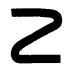
\includegraphics[keepaspectratio]{images/part002_9de8d58d.jpg}}

\begin{enumerate}
\def\labelenumi{\arabic{enumi})}
\setcounter{enumi}{1}
\tightlist
\item
  设 \((\theta_{\alpha})_{\alpha\in\mathbb{A}}\) 是 X 上的一个复测度族；就称族 \((\theta_{\alpha})\) 为可和的，如果正测度族 \((|\theta_{\alpha}|)\) 可和；族 \((\theta_{\alpha})\) 在赋以淡拓扑的向量空间 \(\mathcal{M}(X;\mathbf{C})\) 中可和并不足以保证这一点（参看习题 3）。
\end{enumerate}

\subsection{关于正测度之和的积分}

在本号中，X 表示一个局部紧空间，\((\lambda_{\alpha})_{\alpha\in A}\) 表示 X 上的一个可和正测度族，\(\nu\) 表示测度 \(\sum_{\alpha\in A}\lambda_{\alpha}\) 。

命题 1. --- 设 \(f\) 是定义在 \(X\) 上的一个正数值函数。则

\[
\nu^ {\bullet} (f) = \sum_ {\alpha \in A} \lambda_ {\alpha} ^ {\bullet} (f).\tag{3}
\]

这由注记 1、§1 第 3 号命题 11 及 §1 第 1 号命题 3 立即得出。

推论 1. --- 对 X 的每个紧（相应地，开且相对紧）子集 M，

\[
\nu (\mathrm{M}) = \sum_ {\alpha \in \mathrm{A}} \lambda_ {\alpha} (\mathrm{M}).
\]

推论 2. --- 为使 X 的子集 N 局部 \(\nu\) -可忽略，必须且只须对每个 \(\alpha \in A\) ，N 都是局部 \(\lambda_{\alpha}\) -可忽略的。

推论 3. --- 对每个函数 \(f \in \mathcal{F}_{+}(X)\) ，

\[
\nu^ {*} (f) \geqslant \sum_ {\alpha \in A} \lambda_ {\alpha} ^ {*} (f).\tag{4}
\]

若 \(f\) 不是 \(\nu\) -适度的，则不等式是明显的，因为此时 \(\nu^{*}(f) = +\infty\) （§1 第 2 号命题 7）。若 \(f\) 是 \(\nu\) -适度的，则 \(f\) 是 \(\lambda_{\alpha}\) -适度的（对每个 \(\alpha \in A\) ），因为每个 \(\nu\) -可积开集都是 \(\lambda_{\alpha}\) -可积的；于是关系式 (4) 由 (3) 及 §1 第 2 号命题 7 立即得出。

\pandocbounded{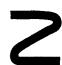
\includegraphics[keepaspectratio]{images/part002_632746ad.jpg}}

即使当 A 可数且每个 \(\lambda_{\alpha}\) 都是点测度时，(4) 的两个成员也可能不相等（ \(\S 1\) 习题 4 \(a\) ））。

命题 2. --- 设 f 是 X 到拓扑空间 G 中的一个映射。为使 f 是 \(\nu\) -可测的，必须且只须 f 是 \(\lambda_{\alpha}\) -可测的（对每个 \(\alpha \in A\) ）。

这由 §1 命题 11 的推论 2 立即得出。

命题 3. --- 为使 X 到 Banach 空间 F 中的映射 f 本质 \(\nu\) -可积，必须且只须 f 本质 \(\lambda_{\alpha}\) -可积（对每个 \(\alpha \in A\) ）且

\[
\sum_ {\alpha \in \mathrm{A}} \int^ {\bullet} | \mathbf {f} | d \lambda_ {\alpha} <   + \infty .\tag{5}
\]

这时族 \((\int \mathbf{f}d\lambda_{\alpha})_{\alpha \in \mathrm{A}}\) 在 \(\mathrm{F}\) 中绝对可和，且

\[
\int \mathbf {f} d \nu = \sum_ {\alpha \in \mathrm{A}} \int \mathbf {f} d \lambda_ {\alpha}.\tag{6}
\]

事实上，为使 \(\mathbf{f}\) 本质 \(\nu\) -可积（相应地，本质 \(\lambda_{\alpha}\) -可积），必须且只须 \(\mathbf{f}\) 对测度 \(\nu\) （相应地，\(\lambda_{\alpha}\) ）可测且 \(\nu^{\bullet}(|\mathbf{f}|) < +\infty\) （相应地，\(\lambda_{\alpha}^{\bullet}(|\mathbf{f}|) < +\infty\) ），这依据 §1 第 3 号命题 9。因而命题的第一部分由命题 2 与命题 1 立即得出。若 \(\mathbf{f}\) 本质 \(\nu\) -可积，则不等式

\[
\sum_ {\alpha \in \mathrm{A}} \left| \int \mathbf {f} d \lambda_ {\alpha} \right| \leqslant \sum_ {\alpha \in \mathrm{A}} \int | \mathbf {f} | d \lambda_ {\alpha} = \nu (| \mathbf {f} |)
\]

表明族 \(\left(\int\mathbf{f}d\lambda_{\alpha}\right)\) 在 F 中绝对可和，且和的范数小于或等于 f 在 \(\overline{\mathcal{L}}_{\mathrm{F}}^{1}(\nu)\) 中的范数。于是满足 (6) 的 \(\mathbf{f}\in\mathcal{L}_{\mathrm{F}}^{1}(\nu)\) 所成之集是 \(\mathcal{L}_{\mathrm{F}}^{1}(\nu)\) 的一个闭线性子空间 H；而这个子空间在 \(\mathcal{L}_{\mathrm{F}}^{1}(\nu)\) 中也是稠密的，因为它包含形如 \(f\cdot a\) 的函数，其中 \(a\in F\) 而 f 表示一个有限可积的正函数（命题 1）。因此 \(\mathcal{H}=\mathcal{L}_{\mathrm{F}}^{1}(\nu)\) ，命题得证。

命题 3 也可由将在 §3（第 3 号定理 1）中证明的关于积分的一般定理导出。

推论 1. --- 设 f 是 \(\nu\) -可积的；则 f 是 \(\lambda_{\alpha}\) -可积的（对每个 \(\alpha \in A\) ），且公式 (6) 成立。反之，若集 A 有限且 f 是 \(\lambda_{\alpha}\) -可积的（对每个 \(\alpha \in A\) ），则函数 f 是 \(\nu\) -可积的。

若 \(\mathbf{f}\) 是 \(\nu\) -可积的，则 \(\mathbf{f}\) 本质 \(\nu\) -可积且 \(\nu\) -适度（§1 第 3 号命题 9 的推论）；因而 \(\mathbf{f}\) 是本质 \(\lambda_{\alpha}\) -可积、\(\lambda_{\alpha}\) -适度从而 \(\lambda_{\alpha}\) -可积的（对每个 \(\alpha \in A\) ）。反之，若 \(A\) 有限且 \(\mathbf{f}\) 是 \(\lambda_{\alpha}\) -可积的（对一切 \(\alpha \in A\) ），则由命题 3，\(\mathbf{f}\) 本质 \(\nu\) -可积，且只需验证 \(\nu^{*}(|\mathbf{f}|) < +\infty\) ；这由关系式 \(\nu^{*} = \sum_{\alpha \in A} \lambda_{\alpha}^{*}\) （第四章，§1 第 3 号命题 15）立即得出。

推论 2. --- 设 \(\theta\) 是 X 上的一个复测度；令 \(\theta_1 = (\mathcal{R}\theta)^+\) ，\(\theta_2 = (\mathcal{R}\theta)^-\) ，\(\theta_3 = (\mathcal{I}\theta)^+\) ，\(\theta_4 = (\mathcal{I}\theta)^-\) 。为使 X 到拓扑空间 G（相应地，到 Banach 空间 F）中的映射 \(f\) 对测度 \(\theta\) 可测（相应地，本质可积、可积），必须且只须它对诸测度 \(\theta_i\) （ \(i = 1,2,3,4\) ）中的每一个都可测（相应地，本质可积、可积）。

若 f 对 \(\theta\) 可测（相应地，本质可积、可积），则按定义 f 对测度 \(|\theta|\) 可测（相应地，本质可积、可积），从而对诸测度 \(\theta_{i}\) （它们都 \(\leqslant |\theta|\) ）也可测（相应地，本质可积、可积）。反之，若 f 对诸测度 \(\theta_{i}\) 可测（相应地，本质可积、可积），则命题 2（相应地，命题 3、命题 3 的推论 1）蕴含 f 对测度 \(\theta_{1} + \theta_{2} + \theta_{3} + \theta_{4}\) （它 \(\geqslant |\theta|\) ）可测（相应地，本质可积、可积）。

\subsection{测度分解为具有紧支集的测度之和}

命题 4. --- 设 \(\mu\) 是局部紧空间 \(T\) 上的一个正测度，并设 \(\mathfrak{K}\) 是紧子集的一个 \(\mu\) -稠密集（\(T\) 的）。存在正测度的一个可和族 \((\mu_{\alpha})_{\alpha \in A}\) （\(T\) 上的），使 \(\mu = \sum_{\alpha \in A} \mu_{\alpha}\) ，且使诸测度 \(\mu_{\alpha}\) 的支集属于 \(\mathfrak{K}\) 并构成两两不相交紧集的一个局部可数族。

若测度 \(\mu\) 是适度的，则可取指标集 A 为可数的。

考虑 K 的两两不相交元素的一个局部可数族 \((\mathrm{K}_{\alpha})_{\alpha\in\mathrm{A}}\) ，使集 \(N = T - \bigcup K_{\alpha}\) 局部 \(\mu\) -可忽略（第四章，§5 第 9 号命题 14）。对每个函数 \(f \in \mathcal{K}(\mathrm{T})\) ，令

\[
\mu_ {\alpha} (f) = \mu (f \varphi_ {\mathrm{K} _ {\alpha}});
\]

线性形式 \(\mu_{\alpha}\) （\(\mathcal{K}(\mathrm{T})\) 上的）是正的，因而是一个正测度，其支集含于 \(\mathrm{K}_{\alpha}\) 。由于含于 \(\mathfrak{K}\) 的一个元素之中的每个紧集都属于 \(\mathfrak{K}\) ，故 \(\operatorname{Supp}(\mu_{\alpha}) \in \mathfrak{K}\) 对一切 \(\alpha \in \mathrm{A}\) 成立。剩下只需证明族 \((\mu_{\alpha})\) 可和且其和等于 \(\mu\) ，换言之，\(\sum_{\alpha \in \mathrm{A}} \mu_{\alpha}(f) = \mu(f)\) 对每个函数 \(f \in \mathcal{K}_{+}(\mathrm{T})\) 成立。设 S 是 \(f\) 的（紧）支集，并设 \(\mathrm{A}'\) 是由 \(\alpha \in \mathrm{A}\) （使 \(\mathrm{S} \cap \mathrm{K}_{\alpha} \neq \varnothing\) 者）组成的可数集。由于集 \(\mathrm{N} \cap \mathrm{S}\) 是 \(\mu\) -可忽略的，

\[
\begin{array}{c} \mu (f) = \mu (f \varphi_ {\mathrm{S}}) = \sum_ {\alpha \in \mathrm{A} ^ {\prime}} \mu (f \varphi_ {\mathrm{S} \cap \mathrm{K} _ {\alpha}}) = \sum_ {\alpha \in \mathrm{A} ^ {\prime}} \mu (f \varphi_ {\mathrm{K} _ {\alpha}}) \\ = \sum_ {\alpha \in \mathrm{A}} \mu (f \varphi_ {\mathrm{K} _ {\alpha}}) = \sum_ {\alpha \in \mathrm{A}} \mu_ {\alpha} (f). \end{array}
\]

这就完成了一般情形的证明。若 \(\mu\) 是适度的，则集 T 是 \(\mu\) -适度的，于是 T 是紧集的一个序列 \((\mathrm{L}_n)\) 与一个可忽略集之并（§1 第 2 号命题 5）；设 \(\mathbf{A}'\) 是由 \(\alpha \in \mathbf{A}\) （使 \(\mathrm{K}_{\alpha}\) 与某个 \(\mathrm{L}_n\) 相交者）组成的可数集。则 \(\mu_{\alpha} = 0\) （对 \(\alpha \notin \mathbf{A}'\) ），而命题的最后一句话立即得证。

注记. --- 一个正测度可能是一个具有紧支集的测度序列之和，而不是适度的（参看 §1 习题 4 a)）。

\section{正测度的积分}

\subsection{取值于测度空间的函数}

设 X 是一个局部紧空间，\(\mathcal{M}_{+}(X)\) 是 X 上正测度所成的凸锥。在本章其余部分，\(\mathcal{M}_{+}(X)\) 总赋有由 \(\mathcal{M}(X)\) 上的淡拓扑诱导的拓扑（第三章，§1 第 9 号）；于是，说映射 \(\Lambda: t \mapsto \lambda_{t}\) （局部紧空间 T 到 \(\mathcal{M}_{+}(X)\) 中的）连续，意思是对每个函数 \(f \in \mathcal{K}(X)\) ，数值函数 \(t \mapsto \lambda_{t}(f)\) 连续。这时我们也称 \(\Lambda\) 在 T 上淡连续。说映射 \(\Lambda: t \mapsto \lambda_{t}\) 是 \(\mu\) -可测的，意思是 T 的紧子集 K （使 \(\Lambda\) 在 K 上的限制淡连续者）所成之集是 \(\mu\) -稠密的（第四章，§5 第 10 号命题 15）。这时我们将称 \(\Lambda\) 是淡 \(\mu\) -可测的。

设 \(\Lambda : t \mapsto \lambda_t\) 是 T 到 \(\mathcal{M}_+(\mathrm{X})\) 中的一个映射；我们就称 \(\Lambda\) 对测度 \(\mu\) 是标量本质可积的，如果对每个函数 \(f \in \mathcal{K}(\mathrm{X})\) ，函数 \(t \mapsto \lambda_t(f)\) 是本质 \(\mu\) -可积的。若令 \(\nu(f) = \int \lambda_t(f) d\mu(t)\) ，则显然 \(\nu\) 是 \(\mathcal{K}(\mathrm{X})\) 上的一个正线性形式，从而是 X 上的一个测度（第三章，§1 第 5 号定理 1）。我们将称 \(\nu\) 为函数 \(\Lambda\) （取值于 \(\mathcal{M}_+(\mathrm{X})\) ）的积分，并写作 \(\nu = \int \lambda_t d\mu(t)\) 。

前面的定义是弱积分概念的一个特例，弱积分将在第六章中以一般方式处理。

若 \(f\) 表示 \(\mathcal{K}(\mathrm{X})\) 的一个元素，则积分 \(\int \lambda_t(f) d\mu(t)\) 滥用记号也可记作 \(\int d\mu(t) \int f(x) d\lambda_t(x)\) ；于是积分 \(\nu = \int \lambda_t d\mu(t)\) 的定义可写成

\[
\int f (x) d \nu (x) = \int d \mu (t) \int f (x) d \lambda_ {t} (x).\tag{1}
\]

在后面，对上积分、本质上积分以及取值于 Banach 空间的函数的积分，我们将作类似的记号滥用。

例. --- 1) 设 T 是一个离散空间，且 \(\mu\) 是在 T 的每个点放置质量 \(+1\) 所定义的 T 上的测度（第三章，§1 第 3 号）。设 \(h\) 是定义在 T 上的一个 \(\geqslant 0\) 的函数；由于函数 \(h\) 在 T 上是下半连续的（甚至是连续的），\(\mu^{*}(h) = \mu^{\bullet}(h) = \sum_{t\in \mathrm{T}}h(t)\) （第四章，§1 第 1 号例）。

对测度 \(\mu\) 而言，可积函数与本质可积函数的概念因此是同一的。在此情形下，说映射 \(t \mapsto \lambda_t\) （T 到 \(\mathcal{M}_+(X)\) 中的）是标量本质 \(\mu\) -可积的，等于说族 \((\lambda_t)_{t \in \mathrm{T}}\) 是可和的（§2 第 1 号），且这时有 \(\int \lambda_t d\mu(t) = \sum_{t \in \mathrm{T}} \lambda_t\) 。注意映射 \(t \mapsto \lambda_t\) 是淡连续的。

\begin{enumerate}
\def\labelenumi{\arabic{enumi})}
\setcounter{enumi}{1}
\tightlist
\item
  映射 \(t \mapsto \varepsilon_t\) （\(T\) 到 \(\mathcal{M}_+(T)\) 中的）是淡连续的、标量本质 \(\mu\) -可积的（\(\mu\) 为 \(T\) 上任一正测度），且有 \(\int \varepsilon_t d\mu(t) = \mu\) 。
\end{enumerate}

命题 1. --- 设 \(\mu\) 是 T 上正测度的一个递增有向族 \((\mu_i)_{i \in I}\) 的上确界；为使 \(\Lambda : t \mapsto \lambda_t\) 是标量本质 \(\mu\) -可积的，必须且只须 \(\Lambda\) 是标量本质 \(\mu_i\) -可积的（对一切 \(i \in I\) ），且族 \(\left( \int \lambda_t d\mu_i(t) \right)_{i \in I}\) 在 \(\mathcal{M}(X)\) 中有上界。这时有，

\[
\int \lambda_ {t} d \mu (t) = \sup _ {i \in \mathrm{I}} \int \lambda_ {t} d \mu_ {i} (t).\tag{2}
\]

因为，验证 \(\Lambda\) 对 T 上一个正测度 \(\eta\) 是标量本质可积的，归结为验证 \(t \mapsto \lambda_{t}(g)\) 是 \(\eta\) -可测的且关于 \(\eta\) 有有限本质上积分（对每个函数 \(g \in \mathcal{K}_{+}(X)\) ）。因而命题由 §1 第 4 号命题 11 及其推论 2 立即得出。

推论. --- 设 \(\mu\) 是正测度的一个可和族 \((\mu_{\alpha})_{\alpha \in \mathbf{A}}\) （\(\mathbf{T}\) 上的）之和；为使 \(\Lambda : t \mapsto \lambda_t\) 是标量本质 \(\mu\) -可积的，必须且只须 \(\Lambda\) 是标量本质 \(\mu_{\alpha}\) -可积的（对每个 \(\alpha \in \mathbf{A}\) ），且测度族 \(\int \lambda_t d\mu_{\alpha}(t)\) 可和。这时有

\[
\int \lambda_ {t} d \mu (t) = \sum_ {\alpha \in A} \int \lambda_ {t} d \mu_ {\alpha} (t).\tag{3}
\]

由此立即得出，每个标量本质 \(\mu\) -可积的映射也都是标量本质 \(\mu'\) -可积的（对每个测度 \(\mu' \leqslant \mu\) ）。

在本节中，我们将限于研究 T 到 \(\mathcal{M}_{+}(X)\) 中的具有下述定义所考虑的性质的标量本质可积映射：

定义 1. --- 设 X 是一个局部紧空间，\(\Lambda : t \mapsto \lambda_t\) 是一个标量本质 \(\mu\) -可积映射（T 到 \(\mathcal{M}_{+}(X)\) 中的），\(\nu\) 是 \(\Lambda\) 的积分。

我们称 \(\Lambda\) 是 \(\mu\) -预适宜的，如果对每个定义在 X 上的下半连续函数 \(f \geqslant 0\) ，函数 \(t \mapsto \int^{\bullet} f d\lambda_t\) 在 T 上 \(\mu\) -可测，且

\[
\int^ {\bullet} f (x) d \nu (x) = \int^ {\bullet} d \mu (t) \int^ {\bullet} f (x) d \lambda_ {t} (x).\tag{4}
\]

我们称 \(\Lambda\) 是 \(\mu\) -适宜的 (*)，如果 \(\Lambda\) 是 \(\mu'\) -预适宜的（对每个正测度 \(\mu' \leqslant \mu\) ）。

可以证明，若 \(\Lambda\) 是 \(\mu\) -预适宜的且测度 \(\nu = \int \lambda_{t} d\mu(t)\) 是适度的——特别地，若 X 在无穷远处可数——则 \(\Lambda\) 是 \(\mu\) -适宜的（习题 7）；然而，尚不知道这两个概念一般是否等价。在下面第 2 与第 3 号的命题叙述中，冠以 a) 或 b) 的断言立即推广到预适宜映射，而冠以 c) 的断言只对适宜映射成立。

下述命题常常使人能验证一个给定的映射是 \(\mu\) -适宜的。

命题 2. --- 设 \(\Lambda : t \mapsto \lambda_t\) 是一个标量本质 \(\mu\) -可积映射（T 到 \(\mathcal{M}_{+}(X)\) 中的），并设 \(\nu = \int \lambda_t d\mu(t)\) 。

\begin{enumerate}
\def\labelenumi{\alph{enumi})}
\tightlist
\item
  若 \(\Lambda\) 是淡连续的，则映射 \(t \mapsto \lambda_t^\bullet(f)\) 对每个定义在 X 上的下半连续函数 \(f \geqslant 0\) 是下半连续的，\(\Lambda\) 是 \(\mu\) -适宜的，且我们有关系式
\end{enumerate}

\[
\int^ {*} f (x) d \nu (x) = \int^ {*} d \mu (t) \int^ {*} f (x) d \lambda_ {t} (x).\tag{5}
\]

\begin{enumerate}
\def\labelenumi{\alph{enumi})}
\setcounter{enumi}{1}
\item
  若 \(\Lambda\) 是淡 \(\mu\) -可测的，则 \(\Lambda\) 是 \(\mu\) -适宜的。
\item
  若 X 的拓扑有可数基，则 \(\Lambda\) 是淡 \(\mu\) -可测的（从而也是 \(\mu\) -适宜的）。
\end{enumerate}

设 \(f\) 是一个 \(\geqslant 0\) 的下半连续函数（定义在 \(X\) 上）。设 \(F\) 是一个对关系 \(\leqslant\) 有向的集，由函数 \(g \in \mathcal{H}(X)\) （满足 \(0 \leqslant g \leqslant f\) ）组成。对 \(g \in F\) ，用 \(h_g\) 表示定义在 \(T\) 上由 \(h_g(t) = \lambda_t(g)\) 给出的函数。类似地，令

\[
h _ {f} (t) = \lambda_ {t} ^ {*} (f) = \lambda_ {t} ^ {\bullet} (f) = \sup _ {g \in \mathrm{F}} h _ {g} (t)
\]

（§1 第 1 号命题 4）。我们作下述比 a) 弱的假设：只设 \(\Lambda\) 在 S 上的限制是淡连续的，其中 S 是 T 的一个包含 \(\mu\) 的支集的闭子集。对 \(g \in \mathbf{F}\) ，用 \(\overline{h}_g\) 表示这样一个数值函数：它在 S 上与 \(h_g\) 相同，且取值 \(+\infty\) 于 \(\mathbb{C}S\) 上。令 \(\overline{h}_f = \sup_{g \in \mathbb{F}} \overline{h}_g\) ；则在 S 上 \(\overline{h}_f = h_f\) 。对每个 \(g \in \mathbf{F}\) ，函数 \(\overline{h}_g\) 是下半连续的；因而 \(\overline{h}_f\) 是下半连续的，且由于族 \((\overline{h}_g)_{g \in \mathbb{F}}\) 是有向的，

\[
\mu^ {*} (\overline {{h}} _ {f}) = \sup _ {g \in \mathrm{F}} \mu^ {*} (\overline {{h}} _ {g}) = \sup _ {g \in \mathrm{F}} \mu^ {*} (h _ {g}) = \sup _ {g \in \mathrm{F}} \nu (g) = \nu^ {*} (f)
\]

（第四章，§1 第 1 号定理 1 及 §2 第 3 号命题 6）。由于在 S 上 \(h_f = \overline{h}_f\) ，从而几乎处处如此，这也可写成 \(\mu^*(h_f) = \nu^*(f)\) ，这是一个与 (5) 恒等的等式。类似地，由于 \(f\) 与 \(\overline{h}_f\) 都是下半连续的，前面的关系式给出等式 \(\mu^\bullet(\overline{h}_f) = \nu^\bullet(f)\) （§1 第 1 号命题 4）；由于在 S 上 \(\overline{h}_f = h_f\) ，由此得出 \(\mu^\bullet(h_f) = \nu^\bullet(f)\) （§1 第 1 号命题 1），这是一个与 (4) 恒等的等式。因此映射 \(\Lambda\) 是 \(\mu\) -预适宜的；但在此论证中处处可把 \(\mu\) 换成 \(\mu' \leqslant \mu\) ，把 \(\nu\) 换成 \(\nu' = \int \lambda_t d\mu'(t)\) ，因为 \(\Lambda\) 也是标量本质 \(\mu'\) -可积的，且 S 包含 \(\mu'\) 的支集。由此得出 \(\Lambda\) 是 \(\mu\) -适宜的。

设 \(\Lambda\) 是淡连续的；可取 \(S = T\) ；则 \(h_f = \overline{h}_f\) 是下半连续的，这就完成了命题 a) 部分的证明。

设 \(\Lambda\) 是淡 \(\mu\) -可测的，我们来证明 b)。集 \(\mathfrak{K}\) （由 T 的紧子集 K （使 \(\Lambda\) 在 K 上的限制连续者）组成）是 \(\mu\) -稠密的（第四章，§5 第 10 号命题 15），故存在 T 上测度的一个可和族 \((\mu_{\alpha})_{\alpha \in \mathrm{A}}\) ，使 \(\mu = \sum_{\alpha \in \mathrm{A}} \mu_{\alpha}\) 且诸测度 \(\mu_{\alpha}\) 中每一个的支集都属于 \(\mathfrak{K}\) （§2 第 3 号命题 4）。对每个 \(\alpha \in \mathrm{A}\) ，映射 \(\Lambda\) 是标量本质 \(\mu_{\alpha}\) -可积的，我们令 \(\nu_{\alpha} = \int \lambda_t d\mu_{\alpha}(t)\) ；族 \((\nu_{\alpha})\) 可和，且其和等于 \(\nu\) （命题 1 的推论）。若 \(f\) 是定义在 X 上的正下半连续函数，则把证明的第一部分应用于测度 \(\mu_{\alpha}\) 与闭集 \(S_{\alpha}\) 就表明：

\(1^{\circ} h_{f}\) 是 \(\mu_{\alpha}\) -可测的（对每个 \(\alpha \in A\) ），从而是 \(\mu\) -可测的（§2 第 2 号命题 2），且

\[
2 ^ {\circ} \int^ {\bullet} f (x) d \nu_ {\alpha} (x) = \int^ {\bullet} d \mu_ {\alpha} (t) \int^ {\bullet} f (x) d \lambda_ {t} (x).
\]

对 \(\alpha\) 求和即得公式 (4)（ \(\S 2\) 第 2 号命题 1）。把前面的论证应用于任意测度 \(\mu' \leqslant \mu\) （这是合法的，因为 \(\Lambda\) 是标量本质 \(\mu'\) -可积且淡 \(\mu'\) -可测的，参看 \(\S 2\) 第 2 号命题 2），我们断定 \(\Lambda\) 是 \(\mu'\) -预适宜的，b) 得证。

最后，设 X 的拓扑有可数基，我们来证明每个标量本质 \(\mu\) -可积映射 \(\Lambda: t \mapsto \lambda_{t}\) （T 到 \(\mathcal{M}_{+}(X)\) 中的）都是淡 \(\mu\) -可测的。这将由下述引理得出：

引理. --- 设 X 是一个有可数基的局部紧空间。则在 \(\mathcal{K}(\mathrm{X})\) 中存在一个可数子集 S，它具有下列性质：对每个函数 \(f \in \mathcal{K}(\mathrm{X})\) ，存在 S 的元素的一个序列 \((f_n)\) 及一个正函数 \(\varphi \in S\) ，使对每个数 \(\varepsilon > 0\) ，只要 n 充分大就有 \(|f_n - f| \leqslant \varepsilon \varphi\) 。

设 \(X'\) 是 \(X\) 的 Alexandroff 紧化，它是一个可度量化紧空间（GT, IX, §2 第 9 号命题 16 及其推论）；我们把 \(\mathcal{K}(X)\) 等同于 \(\mathcal{C}(X')\) 的一个子集。设 \(S'\) 是 Banach 空间 \(\mathcal{C}(X')\) 的一个可数稠密子集（GT, X, §3 第 3 号定理 1）；可设 \(S'\) 包含常函数 \(n\) （对每个 \(n \in N\) ）。设 \((U_n)\) 是 \(X\) 中相对紧开集的一个序列，其并为 \(X\) ，使 \(\overline{U}_n \subset U_{n+1}\) 对一切 \(n\) 成立（GT, I, §9 第 9 号命题 15），并设 \(\varphi_n\) 是 \(\mathcal{K}_+(X)\) 中在 \(\overline{U}_n\) 上等于 1 的函数。我们用 \(S\) 表示 \(\mathcal{K}(X)\) 中形如 \(\varphi_n g\) （ \(n \in N, g \in S'\) ）的元素组成的可数集。若 \(f \in \mathcal{K}(X)\) ，设 \((g_n)\) 是 \(S'\) 的元素的一致收敛于 \(f\) 的一个序列，并设 \(k\) 是使 \(f\) 的支集含于 \(U_k\) 的一个整数。最后，设 \(m\) 是函数 \(g_n\) 的诸范数的一个上界整数。函数 \(f_n = \varphi_k g_n\) 属于 \(S\) 且满足引理的结论，其中 \(\varphi = m\varphi_k\) 。

引理既已建立，且映射 \(t \mapsto \lambda_t(g)\) 是本质 \(\mu\) -可积的（对每个 \(g \in S\) ），故映射 \(t \mapsto (\lambda_t(g))_{g \in S}\) （\(T\) 到 \(\mathbf{R}^S\) 中的）是 \(\mu\) -可测的（第四章，§5 第 3 号定理 1）。于是，集 \(\mathfrak{K}\) （由紧子集 \(K\) （\(T\) 中、使此映射在 \(K\) 上的限制连续者）组成）是 \(\mu\) -稠密的，且只需证明 \(\Lambda\) 在每个 \(K \in \mathfrak{K}\) 上的限制连续。设 \(f\) 是 \(\mathcal{H}(X)\) 的任意元素，\(f_n\) 与 \(\varphi\) 是 \(S\) 中满足引理结论的元素；则函数 \(t \mapsto \lambda_t(f)\) 在 \(K\) 上是连续函数 \(t \mapsto \lambda_t(f_n)\) 的一致极限；因而它在 \(K\) 上连续，命题得证。
